\chapter{Non-Markovian Memory and Causal Simulation}\label{ch:memory}
The construction route is
\[
\text{fractional covariance}\quad\longrightarrow\quad\text{Volterra causality}\quad\longrightarrow\quad\text{Markovian lifting}
\]
The diffusion benchmarks make continuation risk recursive in a small state. Memory breaks that closure in general: two histories can have the same present driver value and different future conditional laws. Fractional covariance describes the target dependence, while Volterra kernels describe how it can be generated from past shocks. Global exact Gaussian sampling and causal sequential simulation therefore answer different computational questions.
\section{Fractional Brownian Motion}


\subsection{Introduction to Markovian Processes and Fractional Brownian Motion}

In stochastic modeling, a fundamental distinction concerns the way in which past information influences future dynamics. In a \textbf{Markovian} framework, the current state of the system is sufficient to describe the probabilistic evolution of the future. Once the present state is known, conditioning on additional information from the remote past does not improve the description of the next transition. In this sense, all relevant historical information is already encoded in the current state.

\begin{definition}[Markov process]
A stochastic process \(\{X_t\}_{t\ge 0}\), adapted to a filtration \(\{\mathcal{F}_t\}_{t\ge 0}\), is said to be \emph{Markovian} if for every \(0\le s<t\) and every measurable set \(A\),
\[
\mathbb{P}(X_t\in A\mid \mathcal{F}_s)
=
\mathbb{P}(X_t\in A\mid X_s).
\]
Equivalently, the conditional law of the future given the whole past depends only on the present state.
\end{definition}

This property is central in many classical stochastic models because it yields a tractable state-space description: one only needs to keep track of the present value \(X_s\), rather than the whole trajectory up to time \(s\).

Fractional Brownian motion departs from this paradigm. Its defining feature is that past increments remain informative about future behavior even over long horizons. As a result, conditioning on the present state alone is not enough to characterize the future evolution. This is the essence of its \textbf{non-Markovian} nature and of its long-memory structure.

\begin{definition}[Non-Markovian process]
A stochastic process is said to be \emph{non-Markovian} if the Markov property fails, that is, if there exist times \(s<t\) for which the conditional law of \(X_t\) given the past \(\mathcal{F}_s\) cannot be reduced to a function of the current state \(X_s\) alone.
\end{definition}

From this perspective, fractional Brownian motion should be viewed as a genuinely \textbf{path-dependent} Gaussian process. The filtration \(\mathcal{F}_t\), representing all information generated by the trajectory up to time \(t\), plays a crucial role because the process carries memory of its past increments. This feature is particularly relevant in financial applications, especially in volatility modeling, where empirical data often exhibit dependence structures that are not well captured by classical Markovian diffusions. Although non-Markovian models are typically more demanding from a computational standpoint, they offer a richer framework for describing persistent or rough temporal behavior.

\subsection{Definition and first properties}

A convenient mathematical entry point to fractional Brownian motion is through its increment process. Rather than starting immediately from the continuous-time covariance kernel, it is useful to first introduce the stationary Gaussian sequence that governs its discrete increments. This sequence is called \emph{fractional Gaussian noise} and represents the fundamental building block of the model.

\begin{definition}[Fractional Gaussian noise]
Let \(H\in(0,1)\). A centered stationary Gaussian sequence
\[
\{X_k\}_{k\in\mathbb{Z}}
\]
is called \emph{fractional Gaussian noise} if its covariance function is
\[
\gamma_H(k)
=
\Cov(X_0,X_k)
=
\frac{1}{2}
\left(
|k+1|^{2H}
-
2|k|^{2H}
+
|k-1|^{2H}
\right),
\qquad k\in\mathbb{Z}.
\]
\end{definition}

The parameter \(H\), called the \emph{Hurst parameter}, governs both the dependence structure of the increments and the roughness of the resulting paths. The benchmark case \(H=\tfrac12\) recovers Gaussian white noise,
\[
\gamma_{1/2}(k)=\delta_{k,0},
\]
so that the increments are uncorrelated and, in the Gaussian setting, independent. When \(H>\tfrac12\), the dependence is predominantly positive and the process is persistent; when \(H<\tfrac12\), the dependence becomes predominantly negative and the process is anti-persistent.

Once the increment sequence has been specified, fractional Brownian motion is obtained by accumulation. On a discrete grid, this means that the process is constructed as the cumulative sum of fractional Gaussian noise.

\begin{definition}[Discrete-time fractional Brownian motion]
Let \(\{X_k\}_{k\ge 1}\) be a fractional Gaussian noise sequence with Hurst parameter \(H\). The associated discrete-time fractional Brownian motion is defined by
\[
B_0^H=0,
\qquad
B_n^H=\sum_{j=1}^{n}X_j,
\qquad n\ge 1.
\]
\end{definition}

Equivalently, on a uniform grid \(t_n=n\Delta t\), one may write
\[
B^H_{t_n}
=
\sum_{j=1}^{n}\Delta B_j^H,
\qquad
\Delta B_j^H:=B^H_{t_j}-B^H_{t_{j-1}},
\]
where, after the appropriate normalization, the increment sequence \(\{\Delta B_j^H\}\) has the covariance structure of fractional Gaussian noise.

The continuous-time version is the canonical Gaussian process associated with this dependence structure.

\begin{definition}[Fractional Brownian motion]
Let \(H\in(0,1)\). A process \(\{B_t^H\}_{t\ge 0}\) is called a \emph{fractional Brownian motion} if it is a centered Gaussian process with covariance function
\[
\Cov(B_s^H,B_t^H)
=
\frac{1}{2}
\bigl(
s^{2H}+t^{2H}-|t-s|^{2H}
\bigr),
\qquad s,t\ge 0.
\]
\end{definition}

Since the process is centered and Gaussian, its law is completely characterized by this covariance kernel. In particular,
\[
\Var(B_t^H)=t^{2H},
\]
so the same parameter \(H\) that governs the dependence of the increments also determines the scaling behavior of the process.

\subsection{Visual comparison across Hurst parameters}

To make the role of the Hurst parameter more transparent, it is useful to compare simulated paths for three benchmark values: \(H=0.2\), \(H=0.5\), and \(H=0.8\). In all panels, the simulation settings are kept fixed, so that the only changing quantity is the Hurst parameter itself. This makes the visual differences directly attributable to the dependence structure induced by \(H\). The precise simulation procedure used to generate these paths, together with the comparison between empirical outputs and theoretical targets, will be introduced in the following sections.

\begin{algorithm}[H]
\caption{Reading the fractional Brownian motion path comparison}
\DontPrintSemicolon
\For{each \(H\in\{0.2,0.5,0.8\}\)}{
  fix the same horizon, grid size, number of paths, and seed structure\;
  generate fractional Gaussian noise with the target covariance\;
  recover \(B^H\) by cumulative summation of the increments\;
  plot the paths and interpret only the change in \(H\)\;
}
\end{algorithm}



\begin{figure}[H]
\centering

%==================== ROW 1 ====================
\begin{minipage}[c][0.24\textheight][c]{0.44\textwidth}
\normalsize
\textbf{Benchmark case: \(H=0.5\).}

This is the reference case corresponding to standard Brownian motion. The increments are independent, so the path displays neither systematic persistence nor systematic mean reversion. Visually, the trajectories fluctuate in an intermediate regime: they are neither excessively jagged nor particularly smooth, and they provide the natural baseline against which the other values of \(H\) should be interpreted.
\end{minipage}
\hfill
\begin{minipage}[c][0.24\textheight][c]{0.50\textwidth}
\centering
\vspace{1.4cm}
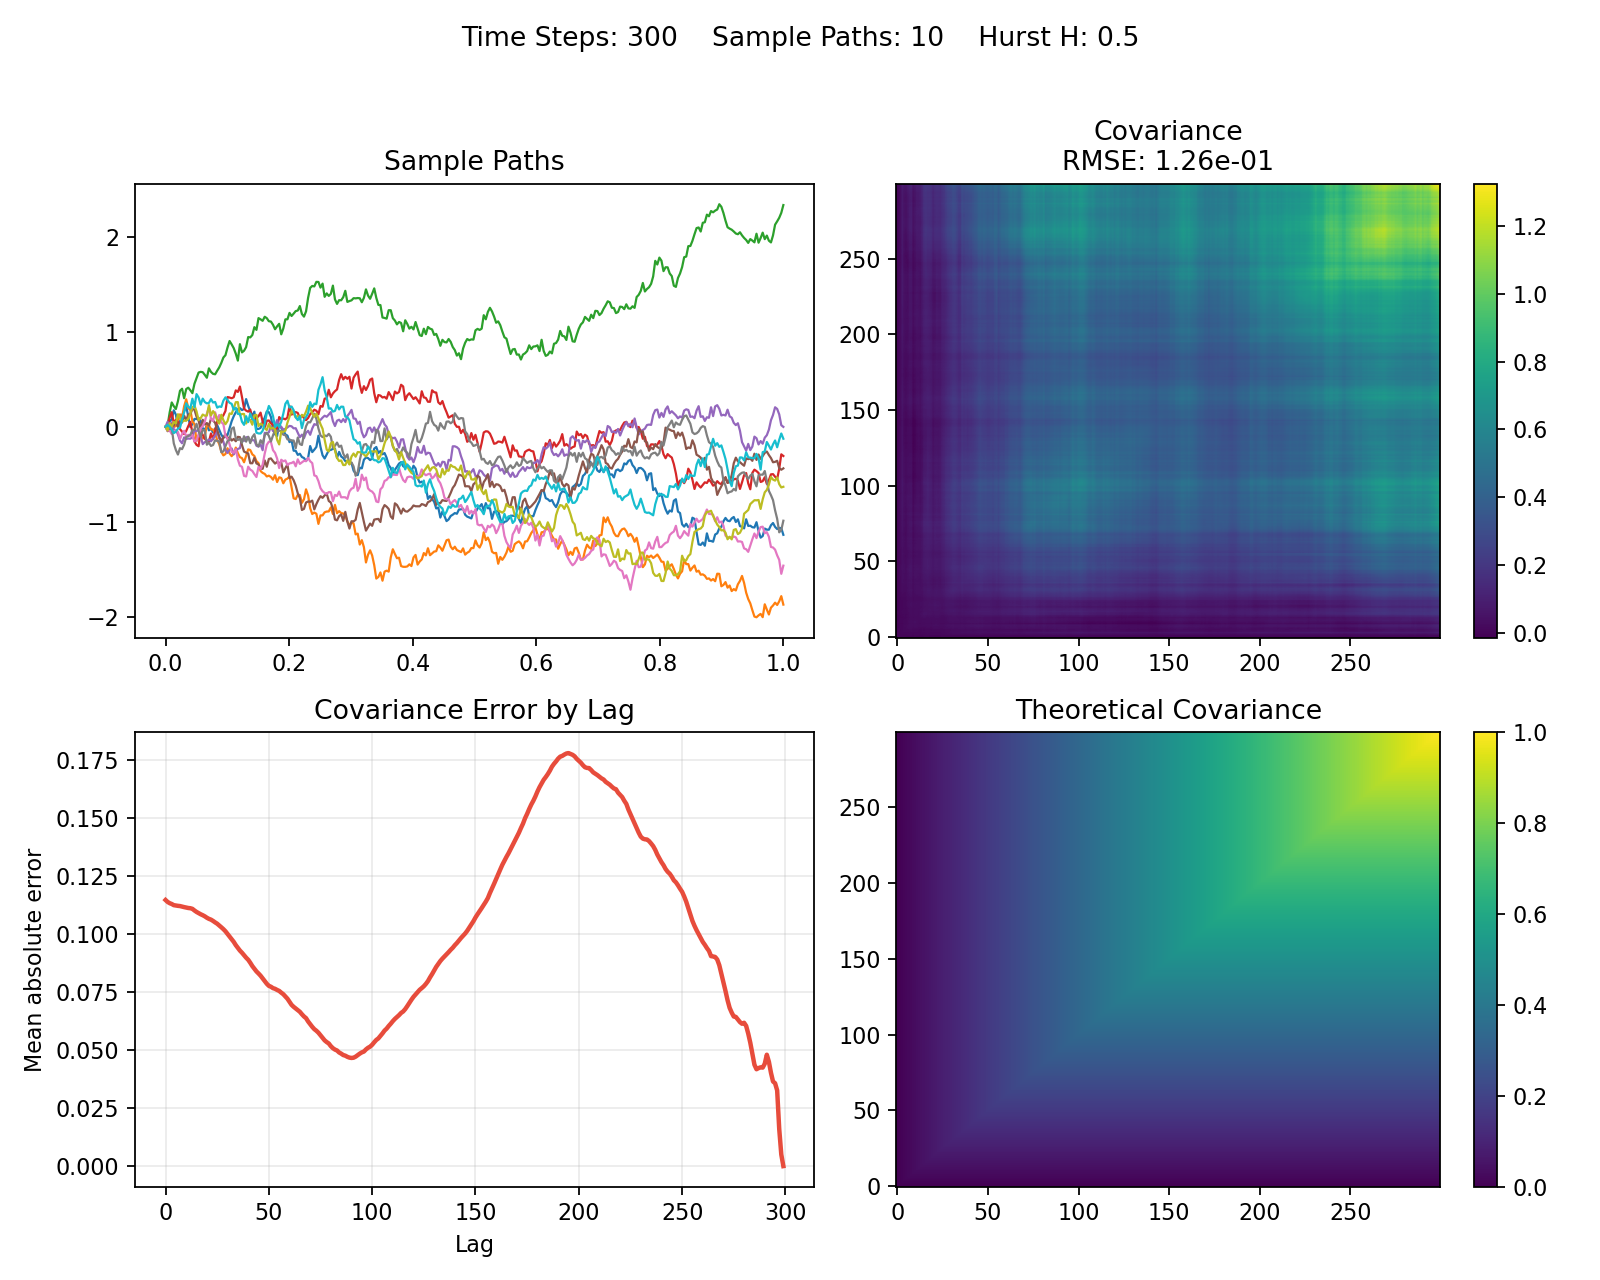
\includegraphics[width=\linewidth]{img/hft2-fgm0_5.png}
\end{minipage}

\vspace{1.2cm}

%==================== ROW 2 ====================
\begin{minipage}[c][0.24\textheight][c]{0.50\textwidth}
\centering
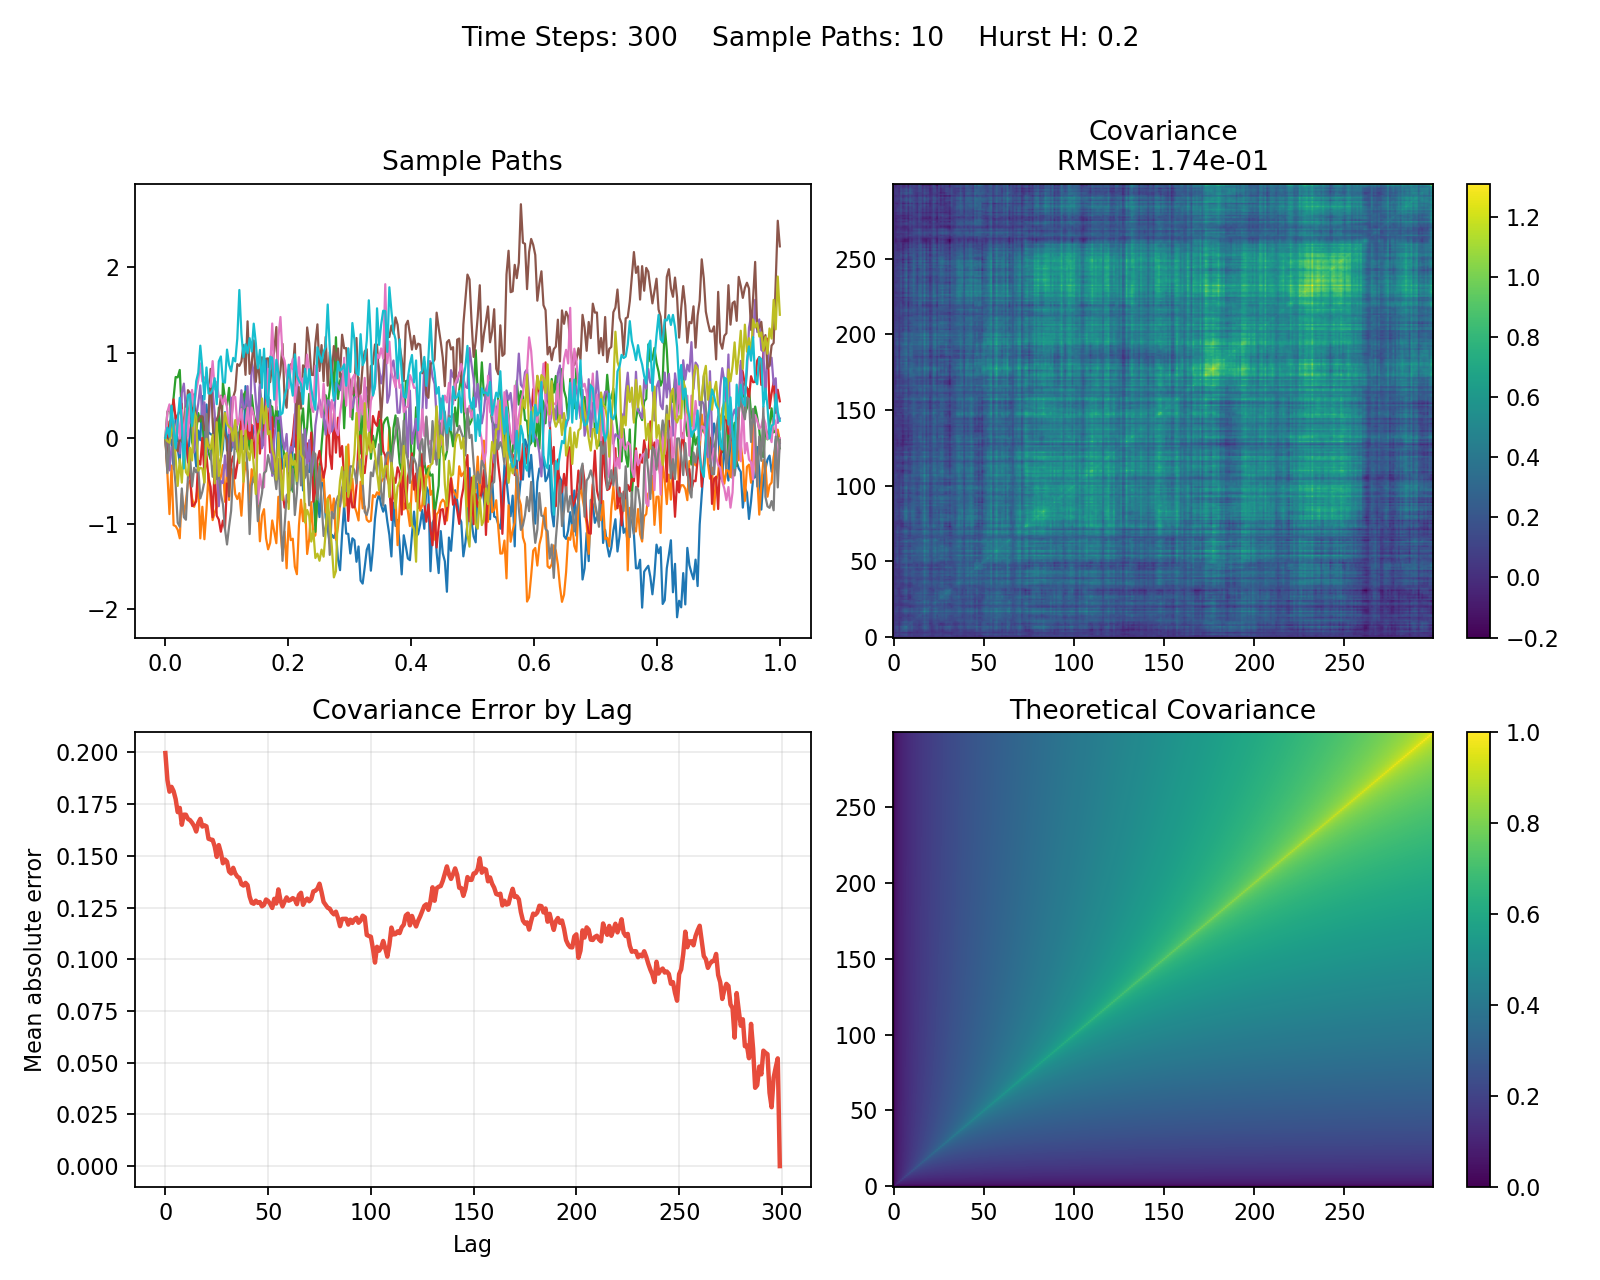
\includegraphics[width=\linewidth]{img/hft2-fgm0_2.png}
\end{minipage}
\hfill
\begin{minipage}[c][0.24\textheight][c]{0.44\textwidth}
\normalsize
\textbf{Anti-persistent regime: \(H=0.2\).}

\vspace{0.3em}

When \(H<\tfrac12\), successive increments tend to have opposite signs. This negative correlation creates a stronger tendency toward local reversals, so the paths appear rougher and more irregular. Compared with the benchmark case \(H=0.5\), the motion oscillates more frequently and displays less local trend continuation. This regime is especially useful when one wants to emphasize roughness and short-term alternation in the trajectory.
\end{minipage}

\vspace{0.8cm}

%==================== ROW 3 ====================
\begin{minipage}[c][0.24\textheight][c]{0.44\textwidth}
\normalsize
\vspace{0.5cm}

\textbf{Persistent regime: \(H=0.8\).}

\vspace{0.3em}

When \(H>\tfrac12\), increments become positively correlated. As a consequence, upward moves are more likely to be followed by upward moves, and downward moves by downward moves. The resulting paths look smoother and more persistent than in the Brownian benchmark. Long local excursions become more visible, and the sample paths exhibit a stronger sense of directional continuity.
\end{minipage}
\hfill
\begin{minipage}[c][0.24\textheight][c]{0.50\textwidth}
\centering
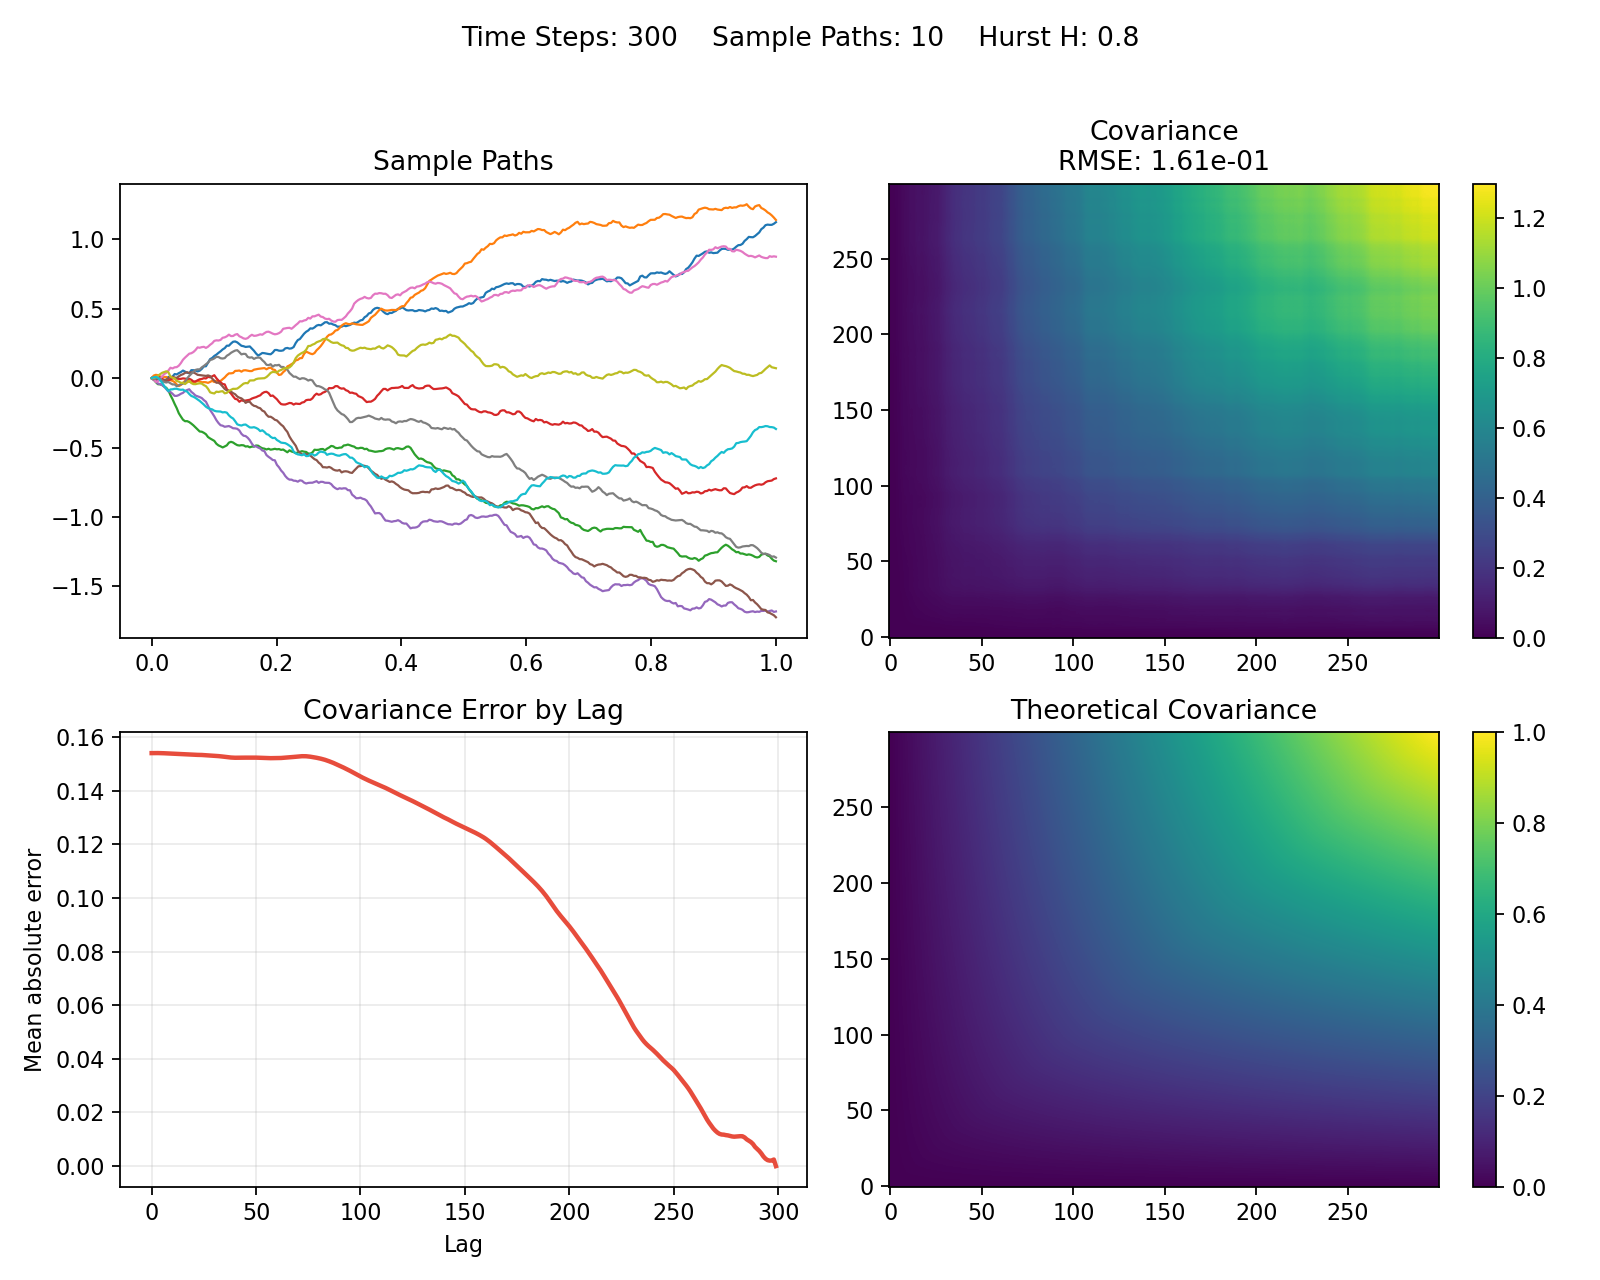
\includegraphics[width=\linewidth]{img/hft2-fgm0_8.png}
\end{minipage}

\end{figure}

\vspace{0.5cm}

\subsection{Financial applications and computational challenges}

The interest in fractional Brownian motion within quantitative finance is mainly motivated by its ability to encode temporal dependence beyond the Markovian paradigm. In particular, when volatility is modeled as a latent process rather than as a directly traded asset, long-memory or roughness effects can become empirically relevant. This is one of the reasons why fractional-type models, and especially rough-volatility specifications, have attracted growing attention in the literature.

A natural interpretation of this point arises through the dynamics of log-volatility. If volatility exhibits dependence across multiple time scales, then a path-dependent Gaussian driver may provide a richer description than standard Brownian motion. In rough-volatility applications, this motivates the use of non-Markovian Gaussian structures to capture irregular short-term behavior together with persistent dependence.

This additional realism, however, comes at a cost. Once volatility is driven by a non-Markovian process, the model no longer admits the simple low-dimensional state representation available in classical diffusion frameworks. As a consequence, pricing and calibration become substantially more expensive. If one wishes to fit such a model to an implied-volatility surface, the procedure typically requires repeated simulation of the full volatility path, followed by repeated pricing across a grid of strikes and maturities.

The difficulty is not limited to pricing alone. Calibration requires solving an inverse problem: one must search over a parameter space until the model-generated prices or implied volatilities match the observed surface. In a non-Markovian setting, each candidate parameter vector may require a full path simulation, making the overall procedure too costly for live or large-scale applications.

This trade-off has motivated a parallel line of research based on surrogate methods. Instead of rerunning the full pricing model at each calibration step, one can attempt to learn the map from model parameters to implied-volatility surfaces through neural networks or other machine-learning approximators. If successful, such a surrogate can dramatically accelerate calibration. At the same time, the gain in speed comes with its own issues: approximation error, limited extrapolation power, and the fact that desirable structural properties, such as no-arbitrage consistency, are not automatically guaranteed.

For this reason, fractional Brownian motion should be viewed not as a free improvement over standard models, but as a richer modeling choice that trades analytical tractability for empirical flexibility. This trade-off makes simulation methodology especially important. We therefore begin with the Davies--Harte construction, which is a convenient way to generate fractional Gaussian noise and fractional Brownian motion with the correct covariance structure.

\subsection{Davies--Harte Simulation and Validation}

The trajectories displayed in the visual comparison above are most naturally generated from the increment process rather than from a direct covariance factorization. Among the available simulation methods, the Davies--Harte scheme is particularly convenient because it is both mathematically transparent and computationally efficient: it generates fractional Gaussian noise by embedding its covariance sequence into a circulant structure diagonalized by the FFT, and then recovers fractional Brownian motion by cumulative summation.

\paragraph{Inputs.} The basic inputs of the scheme are
\[
H\in(0,1), \qquad T>0, \qquad N\in\mathbb{N},
\]
where \(H\) is the Hurst parameter, \(T\) is the terminal time, and \(N\) is the number of time steps. We also define
\[
\Delta t = \frac{T}{N},
\qquad
t_n = n\Delta t,
\qquad n=0,1,\dots,N.
\]
Increasing \(N\) refines time resolution. Agreement of empirical covariance with its theoretical target also depends on path count, validity of the embedding and sampling error; time-grid refinement alone does not guarantee closer empirical statistics.

\paragraph{Step 1: generate the time grid.} The first step is to discretize the interval \([0,T]\):
\[
t_n=n\Delta t,
\qquad n=0,1,\dots,N.
\]
This produces the \(N+1\) points on which the path will be represented.

\paragraph{Step 2: define the autocovariance of fractional Gaussian noise.} The Davies--Harte construction works directly with fractional Gaussian noise. Its autocovariance is
\[
\gamma_H(k)
=
\frac{1}{2}
\left(
|k+1|^{2H}
-
2|k|^{2H}
+
|k-1|^{2H}
\right),
\qquad k\in\mathbb{Z}.
\]
This formula determines the dependence structure of the increments and is the starting point of the whole algorithm.

\paragraph{Step 3: build the circulant covariance vector.} The key idea is to embed the covariance sequence into a circulant vector of length \(2N\). One convenient choice is
\[
c=
\bigl(
\gamma_H(0),\gamma_H(1),\dots,\gamma_H(N-1),0,
\gamma_H(N-1),\dots,\gamma_H(1)
\bigr).
\]
This step is crucial because circulant matrices are diagonalized by the discrete Fourier transform, which makes the method computationally efficient.

\paragraph{Step 4: compute the embedded eigenvalues via FFT.} Let
\[
m=2N.
\]
Applying the FFT to the circulant vector produces the embedded eigenvalues
\[
\lambda_j=\Re\bigl(\mathrm{FFT}(c)_j\bigr),
\qquad j=0,\dots,m-1.
\]
Since this is a covariance embedding, the relevant eigenvalues must be nonnegative up to numerical tolerance. In practice, one checks this explicitly before proceeding.

\paragraph{Step 5: generate the complex Gaussian vector.} The next step is to construct a complex Gaussian vector \(Z=(Z_0,\dots,Z_{m-1})\) with the conjugate symmetry required by the inverse transform. Let \(\xi_k,\eta_k\) be independent standard normal random variables. Then define
\[
Z_0=\sqrt{\lambda_0}\,\xi_0,
\qquad
Z_N=\sqrt{\lambda_N}\,\xi_N,
\]
and for \(k=1,\dots,N-1\),
\[
Z_k
=
\sqrt{\frac{\lambda_k}{2}}
\left(\xi_k+i\eta_k\right),
\qquad
Z_{m-k}=\overline{Z_k}.
\]
This is the most delicate part of the scheme. The conjugate assignment ensures that the inverse FFT will return a real-valued Gaussian sequence.

\paragraph{Step 6: apply the inverse FFT and restore the time scale.} Applying the inverse FFT to \(Z\) produces a realization of fractional Gaussian noise. However, one must be careful with scaling. In NumPy, the inverse FFT includes a factor \(1/m\), so a correction is needed. In addition, the correct time scale must be restored through \(\Delta t^H\). The simulated increments are therefore
\[
\Delta B_j^H
=
\Delta t^H\,\sqrt{m}\,
\Re\!\left(\mathrm{IFFT}(Z)_j\right),
\qquad j=0,\dots,N-1.
\]
The factor \(\sqrt{m}\) corrects the normalization introduced by the inverse FFT, while \(\Delta t^H\) ensures that
\[
\Var(\Delta B_j^H)=\Delta t^{2H}.
\]

\paragraph{Step 7: recover fractional Brownian motion by cumulative summation.} Once the increments have been generated, fractional Brownian motion is obtained by accumulation:
\[
B_0^H=0,
\qquad
B_{t_n}^H=\sum_{j=0}^{n-1}\Delta B_j^H,
\qquad n=1,\dots,N.
\]
This final step is conceptually simple but essential: the whole simulation procedure reduces to generating the correct correlated Gaussian increments and summing them.

\subsection{Simulation and confirmation against theoretical results}

Once the simulation scheme has been implemented, the next question is whether the output is actually correct. A plausible-looking path is not enough: even a small scaling mistake inside the FFT or inverse FFT can generate visually convincing trajectories whose empirical moments do not match the theoretical ones. For this reason, the simulation should be validated against the variance of fractional Gaussian noise, the variance of fractional Brownian motion, and the full covariance kernel of the process.

\paragraph{Variance of the increments and of the process.} The most immediate diagnostic consists in comparing empirical and theoretical variances. For the simulated fractional Gaussian noise, the theoretical variance is
\[
\Var(\Delta B_j^H)=\Delta t^{2H}.
\]
For fractional Brownian motion itself, the variance at time \(t_n\) is
\[
\Var(B_{t_n}^H)=t_n^{2H}.
\]
These two identities provide a simple but informative consistency check. The first confirms that the increment process has been scaled correctly, while the second confirms that the cumulative summation from fractional Gaussian noise to fractional Brownian motion has been implemented properly.

In practice, one generates many paths, computes empirical variances, and compares them to the theoretical targets. As the number of simulated paths and the grid resolution increase, the discrepancy should decrease.

\paragraph{Covariance-matrix confirmation.} A more informative validation compares the full empirical covariance matrix of the simulated process to the theoretical covariance kernel
\[
\Gamma_{ij}
=
\Cov(B_{t_i}^H,B_{t_j}^H)
=
\frac12\left(
t_i^{2H}+t_j^{2H}-|t_i-t_j|^{2H}
\right).
\]
Given \(M\) simulated paths \(B^{(1)},\dots,B^{(M)}\), one can estimate the empirical covariance matrix by
\[
\widehat{\Gamma}_{ij}
=
\frac{1}{M-1}
\sum_{r=1}^{M}
\left(B_{t_i}^{(r)}-\overline{B}_{t_i}\right)
\left(B_{t_j}^{(r)}-\overline{B}_{t_j}\right),
\]
where \(\overline{B}_{t_i}\) is the empirical mean at time \(t_i\). The discrepancy between empirical and theoretical covariance can then be summarized by the root mean squared error
\[
\mathrm{RMSE}
=
\left(
\frac{1}{(N+1)^2}
\sum_{i=0}^{N}\sum_{j=0}^{N}
\bigl(\widehat{\Gamma}_{ij}-\Gamma_{ij}\bigr)^2
\right)^{1/2}.
\]

This is the natural theoretical benchmark for the simulated paths shown earlier. The visual comparison in the previous figure illustrates how the geometry of the trajectories changes with \(H\); the covariance validation presented here explains why those paths are statistically consistent with the definition of the process.

\paragraph{Error decay in \(N\) and \(M\).} A correct implementation should not only reproduce the covariance structure at one fixed parameter choice, but should also exhibit the expected improvement as the numerical inputs increase. There are two natural directions along which to check this.

First, increasing \(N\) refines the time grid and improves the empirical representation of the increment process. In particular, one may study how the RMSE associated with the variance of fractional Gaussian noise decreases as the grid becomes finer.

Second, increasing the number of simulated paths \(M\) improves the empirical estimation of the covariance matrix. Since covariance estimation is a Monte Carlo object, the RMSE should decay at the standard rate
\[
\mathrm{RMSE}=O(M^{-1/2}).
\]
This provides a useful benchmark: if the implementation is correct, increasing the sample size should reduce the covariance estimation error approximately at that rate.


\begin{algorithm}[H]
\caption{Validation diagnostics before the convergence figure}
\DontPrintSemicolon
\For{each grid size \(N\)}{
  simulate fractional Gaussian noise and compare empirical increment variance with \(\Delta t^{2H}\)\;
}
\For{each number of paths \(M\)}{
  estimate the empirical covariance matrix of \(B^H\)\;
  compare it with the theoretical covariance kernel and record the RMSE\;
}
plot both error curves against their theoretical decay benchmarks\;
\end{algorithm}

\begin{figure}[H]
\centering
\begin{minipage}[t]{0.48\textwidth}
\centering
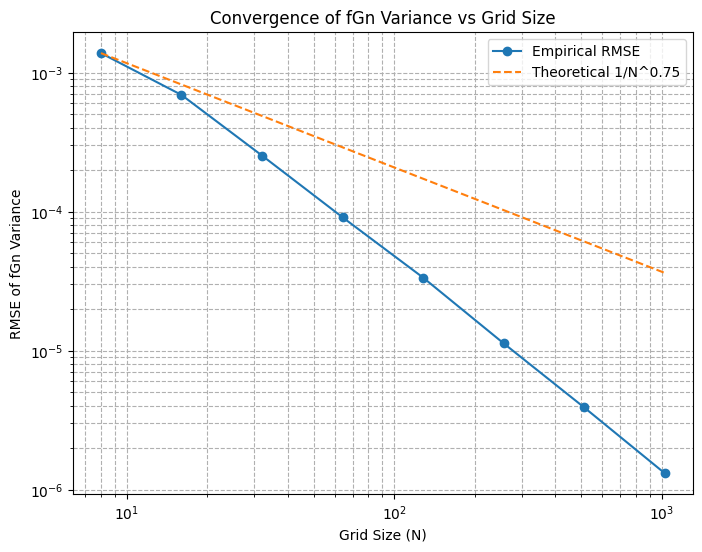
\includegraphics[width=\linewidth]{img/hft2-img_4.png}
\end{minipage}
\hfill
\begin{minipage}[t]{0.48\textwidth}
\centering
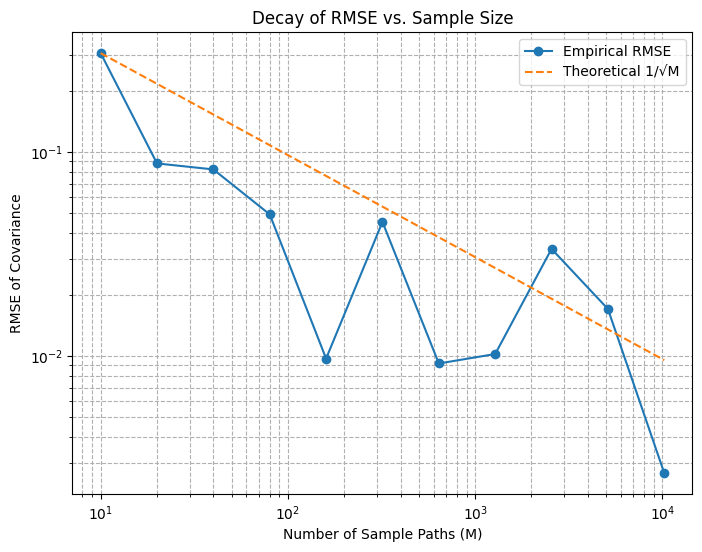
\includegraphics[width=\linewidth]{img/hft2-img_5.png}
\end{minipage}
\caption{Convergence diagnostics for the Davies--Harte implementation. The left panel compares the empirical decay of the RMSE for the variance of fractional Gaussian noise with the theoretical benchmark as the grid size \(N\) increases. The right panel compares the empirical decay of the covariance RMSE with the Monte Carlo reference rate \(1/\sqrt{M}\) as the number of simulated paths \(M\) grows.}
\label{hft2-fig:fbm_convergence_diagnostics}
\end{figure}

Taken together, these checks provide a coherent validation strategy. First, one verifies that the increment process and the accumulated process have the correct variance scaling. Then, one compares the full empirical covariance matrix to the theoretical covariance kernel. Finally, one checks that the numerical error decreases in the expected way as \(N\) and \(M\) increase. Figure \ref{hft2-fig:fbm_convergence_diagnostics} illustrates these convergence patterns directly. The decay in the left panel is consistent with improved variance accuracy on finer grids, while the right panel shows the expected overall reduction in covariance error as the sample size increases, despite the visible finite-sample noise typical of Monte Carlo experiments.

\subsection{Problems of Davies--Harte simulations}

The Davies--Harte scheme is an elegant and efficient way to generate fractional Gaussian noise and, by cumulative summation, fractional Brownian motion. For offline Monte Carlo experiments it is extremely useful, since it reproduces the target covariance structure accurately and does so at relatively low computational cost. For the purposes of this study, however, this efficiency comes with an important limitation: the construction is fundamentally global rather than causal.

The issue is not that fractional Brownian motion itself depends on future information. It does not. The issue is instead numerical and structural. In the Davies--Harte scheme, one fixes the entire time grid in advance, embeds the covariance sequence into a circulant structure, applies spectral methods, and generates the full trajectory at once. In this sense, the algorithm requires \emph{global path knowledge}: the desired covariance structure is enforced through a construction that acts on the whole path simultaneously, rather than through a recursive state update based only on past shocks.

This point matters in sequential financial applications. In market making, filtering, and related control problems, one typically wants a representation that evolves forward in time as new information arrives. At each time \(t\), the state should be updated causally from what is already known, without relying on a simulation architecture that is tied to the full terminal horizon. From this perspective, Davies--Harte is mathematically valid and computationally efficient, but it is not the most natural language for an online control problem.

A related limitation appears in model fitting. If one were to use a non-Markovian volatility specification driven by fractional Brownian motion and calibrate it to an implied-volatility surface, then in the absence of a closed-form pricing formula one would typically need repeated Monte Carlo simulation. For each parameter choice, one must simulate the full volatility path, generate prices over a grid of strikes and maturities, compare the model output with the observed surface, and then iterate over the parameter space. Even if the underlying simulator is efficient, this overall calibration loop quickly becomes computationally intensive and may become impractical in a live setting.

There is therefore a genuine trade-off. On the one hand, rough or long-memory dynamics may capture empirically relevant dependence structures more faithfully than classical Markovian diffusions. On the other hand, these gains do not come for free: they are purchased with greater numerical cost and with the loss of a simple recursive state representation. In particular, while Davies--Harte is well suited for global path generation and covariance-based validation, it is not the most convenient framework when the final objective is a causal simulation architecture for sequential pricing or inventory control.

For these reasons, the Davies--Harte scheme should be regarded as an excellent benchmark for simulation and validation, but not yet as the most natural representation for control-oriented modeling. What is needed next is a formulation that preserves memory while making causality explicit. This is precisely the role of Gaussian Volterra processes: they replace the global covariance viewpoint with a kernel-based construction in which the state at time \(t\) depends on past noise only. This makes them a more natural starting point for rough-volatility simulation, approximation, and eventually market-making control.

%%%%%%%%%%%%%%%%%%%%%%%%%%%%%%%%%%%%%%%%%%%%%%%%
%%%%%%%%%%%%%%%%%%%%%%%%%%%%%%%%%%%%%%%%%%%%%%%%
%%%%%%%%%%%%%%%%%%%%%%%%%%%%%%%%%%%%%%%%%%%%%%%%

\section{Volterra Gaussian Processes and Causality}


\paragraph{From global covariance to causal kernels.}

Given a Brownian driver, the Volterra kernel assigns a weight to every shock that is already observable at time \(t\). This separates two roles that a covariance-first simulator leaves implicit: the support condition determines which shocks may enter the state, while the kernel profile determines their relative influence. That distinction is useful in a pricing engine or control loop because it exposes the information set used by each update.

This is the main difference with covariance-based simulation methods such as Davies--Harte. There, the objective is to sample the entire path with the correct law, and this is done through a global embedding of the covariance sequence. In a Volterra representation, by contrast, one builds the process forward in time through a weighted accumulation of Brownian shocks. The weights are determined by the kernel, and therefore the kernel becomes the object that controls both the dependence structure and the geometry of the paths.

\subsection{General Volterra representation}

\begin{definition}[Gaussian Volterra process]
Let \(W\) be a standard Brownian motion and let \(K(t,s)\) be a measurable kernel such that
\(
K(t,s)=0 \; \text{for } s>t,
\; \text{and}  \;
\int_0^t K(t,s)^2\,ds<\infty
\; \text{for all } t\ge 0.
\)
A \emph{Gaussian Volterra process} is a process of the form
\[
X_t=\int_0^t K(t,s)\,dW_s.
\]
\end{definition}

The condition \(K(t,s)=0\) for \(s>t\) is the mathematical expression of causality: the process at time \(t\) depends only on shocks observed before time \(t\). The entire covariance structure is therefore encoded in the kernel itself.

\subsection{Covariance induced by the kernel}

The key step is to show how the kernel determines the covariance of the process. Since the stochastic integral is centered, one expects the covariance to reduce to an expectation of a product of integrals, which can then be simplified by It\^o isometry.

\begin{proposition}[Covariance induced by a Volterra kernel]
Let
\[
X_t=\int_0^t K(t,s)\,dW_s.
\]
Then for any \(s,t\ge 0\),
\[
\Cov(X_s,X_t)
=
\int_0^{s\wedge t} K(s,u)K(t,u)\,du.
\]
\end{proposition}

\begin{proof}
Since \(X_s\) and \(X_t\) are centered Gaussian variables,
\[
\Cov(X_s,X_t)=\E[X_sX_t].
\]
Using the stochastic integral representation,
\[
\E[X_sX_t]
=
\E\!\left[
\left(\int_0^s K(s,u)\,dW_u\right)
\left(\int_0^t K(t,v)\,dW_v\right)
\right].
\]
By It\^o isometry for products of stochastic integrals,
\[
\E\!\left[
\left(\int_0^s f(u)\,dW_u\right)
\left(\int_0^t g(v)\,dW_v\right)
\right]
=
\int_0^{s\wedge t} f(u)g(u)\,du.
\]
Applying this with \(f(u)=K(s,u)\) and \(g(u)=K(t,u)\) gives
\[
\Cov(X_s,X_t)
=
\int_0^{s\wedge t} K(s,u)K(t,u)\,du. \qedhere
\]
\end{proof}
    
This identity is the central bridge between the process and its second-order structure. It shows that once the kernel is selected, the covariance is no longer imposed externally: it is generated mechanically by the causal accumulation of Brownian shocks.

\paragraph{Why causality matters.}

The formula above also explains why the upper integration limit becomes \(s\wedge t\). If \(u>s\), then \(K(s,u)=0\) by causality; similarly, if \(u>t\), then \(K(t,u)=0\). Hence the product \(K(s,u)K(t,u)\) can only be nonzero when \(u\le s\) and \(u\le t\), which is equivalent to \(u\le s\wedge t\).

This point is important in sequential financial applications. In an online control problem one does not want a representation that is tied to the whole terminal horizon or to a global covariance embedding. Instead, one wants a state variable that can be updated as new information arrives. A Volterra process has exactly this interpretation: it is built from past noise only, with the memory of the process encoded through the kernel.

At the same time, causality should not be confused with Markovianity. A causal Volterra process may still be strongly non-Markovian. The value at time \(t\) does not depend on future noise, but it may depend on the entire past history of the driving Brownian motion. This is precisely what makes Volterra processes flexible enough to reproduce both rough and persistent behavior.

\subsection{Discretization and non-Markovian structure}

Once the Volterra representation is available, discretization is conceptually simple. Fix a horizon \(T>0\) and choose a uniform grid
\(
0=t_0<t_1<\cdots<t_n=T,
\quad
t_i=\frac{iT}{n},
\quad
\Delta t=\frac{T}{n}.
\)
Let
\[
\Delta W_j = W_{t_{j+1}}-W_{t_j},
\quad
\Delta W_j\sim \mathcal{N}(0,\Delta t),
\]
with independent increments across \(j\). A Riemann--It\^o approximation of the stochastic integral then yields
\[
X_{t_i}
\approx
\sum_{j=0}^{i-1} K(t_i,t_j)\,\Delta W_j.
\]

This discrete expression is the natural simulation recipe: choose a kernel, generate Brownian increments, and at each time point accumulate the past shocks with the appropriate weights. After the grid values have been obtained, one may visualize the path through piecewise linear interpolation, which is simply the numerical analogue of joining the dots.

\paragraph{Iterative construction.}

The discretized Volterra process can be built step by step from left to right. At the first nonzero grid point,
\[
X_{t_1}\approx K(t_1,t_0)\,\Delta W_0.
\]
At the next step,
\[
X_{t_2}\approx K(t_2,t_0)\,\Delta W_0 + K(t_2,t_1)\,\Delta W_1,
\]
and more generally
\[
X_{t_i}\approx \sum_{j=0}^{i-1} K(t_i,t_j)\,\Delta W_j.
\]

This already makes the causal structure visible: to build \(X_{t_i}\), one needs only the Brownian increments observed before time \(t_i\). But the same formula also shows why the process is non-Markovian in general. Indeed, the increment from \(t_{i-1}\) to \(t_i\) is
\[
X_{t_i}-X_{t_{i-1}}
\approx
K(t_i,t_{i-1})\,\Delta W_{i-1}
+
\sum_{j=0}^{i-2}
\bigl(K(t_i,t_j)-K(t_{i-1},t_j)\bigr)\,\Delta W_j.
\]
Unless the kernel is trivial, the new increment depends not only on the most recent shock, but also on the entire path history through all previous \(\Delta W_j\). This is exactly the discrete manifestation of non-Markovianity.

The special case in which this dependence disappears is standard Brownian motion. If one chooses the trivial kernel
\(
K(t,s)=1,
\; 0\le s<t,
\)
then
\[
X_t=\int_0^t dW_s = W_t,
\]
and the increment structure collapses to the familiar Markovian setting. This observation is useful: the Volterra framework contains Brownian motion as a limiting benchmark, but becomes genuinely non-Markovian as soon as the kernel introduces memory.
\subsection{Representative kernels and induced dynamics}

The flexibility of the Volterra representation comes from the choice of kernel. Different kernels induce different covariance structures and therefore different path dynamics.

\textbf{Brownian kernel}

The simplest example is
\(
K_{\mathrm{BM}}(t,s)=1.
\)
This reproduces standard Brownian motion,
\[
X_t=\int_0^t dW_s=W_t.
\]
In this case the Volterra construction is mathematically correct but computationally unnecessary, since Brownian motion can be simulated directly from independent Gaussian increments. Its main value here is conceptual: it shows that a Markovian process is contained as a special case in the broader Volterra family.

\textbf{Exponential kernel and mean reversion}

A second important example is the exponential kernel
\[
K_{\theta}(t,s)=e^{-\theta(t-s)}\mathbf{1}_{\{0\le s<t\}},
\qquad \theta>0.
\]
This kernel generates the Ornstein--Uhlenbeck process
\[
X_t=\int_0^t e^{-\theta(t-s)}\,dW_s,
\]
which solves the mean-reverting stochastic differential equation
\[
dX_t=-\theta X_t\,dt + dW_t.
\]
The exponential decay gives more weight to recent shocks than to distant ones, producing the familiar pull back toward the mean.

\textbf{Fractional-type kernel and roughness}

The rough-volatility literature is driven by singular power-law kernels. A simple causal prototype is
\[
\widetilde{K}_H(t,s)
=
\sqrt{c_H}\,(t-s)^{H-\frac12}\mathbf{1}_{\{0\le s<t\}},
\qquad
c_H=\frac{\Gamma(2H+1)}{2\,\Gamma(H+\frac12)^2},
\]
with \(H\in(0,1)\). The kernel is singular near the diagonal \(t=s\), which means that very recent history receives a particularly large weight. This is what generates roughness when \(H<\tfrac12\) and smoother, more persistent behavior when \(H>\tfrac12\). In the diagnostic implementation, the boundary value \(H=\tfrac12\) is treated separately with the exact Brownian kernel \(K(t,s)=\mathbf{1}_{\{s<t\}}\), so the resulting process is standard Brownian motion rather than the limiting normalization of this prototype.

\begin{remark}[Exact versus simplified fractional kernels]
Standard fractional Brownian motion admits an exact Volterra representation with a kernel \(K_H(t,s)\), but the closed form is more involved than a simple power law. In numerical intuition and in many rough-volatility approximations, one instead works with a tractable causal power-law kernel whose local behavior reproduces the desired roughness exponent. This chapter follows that practical route, since the goal is to prepare a simulation architecture rather than a complete classification of exact Gaussian representations.
\end{remark}

\subsection{Visual comparison across Hurst parameters}

The effect of the kernel is easiest to understand visually. In the panels below, the left block for each value of \(H\) illustrates the iterative construction of the process through a filtration window: as the window expands, the path is built using progressively more past information, exactly as required by causality. The right block shows the corresponding Volterra diagnostics, including sample paths, the kernel heat map, the Brownian driver, the full support of representative kernel slices, and the covariance induced by the discrete kernel. The reported RMSE compares that induced covariance with the standard fractional-Brownian target; it is zero up to numerical precision in the Brownian benchmark and need not vanish for the simplified power-law kernels.

\begin{algorithm}[H]
\caption{Reading the Volterra construction panels}
\DontPrintSemicolon
choose a causal kernel \(K_H(t,s)\) and Brownian increments \(\Delta W_j\)\;
\For{each time index \(i\)}{
  compute \(X_{t_i}\approx\sum_{j<i}K_H(t_i,t_j)\Delta W_j\) using past shocks only\;
  reveal the filtration window that is available at that step\;
}
plot the iterative path construction beside the kernel, noise, causality, and covariance diagnostics\;
\end{algorithm}



\begin{figure}[H]
\vspace{0cm}
\centering
\begin{minipage}[t]{0.44\textwidth}
\vspace{0cm}
\normalsize


\textbf{Benchmark regime: \(H=0.5\).}

The value \(H=\tfrac12\) is the exact Brownian benchmark. Here \(K(t,s)=1\) for \(s<t\) and \(K(t,s)=0\) for \(s\ge t\), so each kernel slice is flat over the observed past and drops to zero over the future. Consequently \(X_t=\int_0^t dW_s=W_t\): disjoint increments are independent and there is no fractional memory, although the construction remains causal because no future shock enters the state. The kernel heat map and the covariance heat map use the same numerical color range \([0,1]\), but their shapes differ by construction: the first is the binary support kernel, while the second is \(\Cov(W_t,W_s)=\min(t,s)\).

\vspace{0.5cm}
\centering
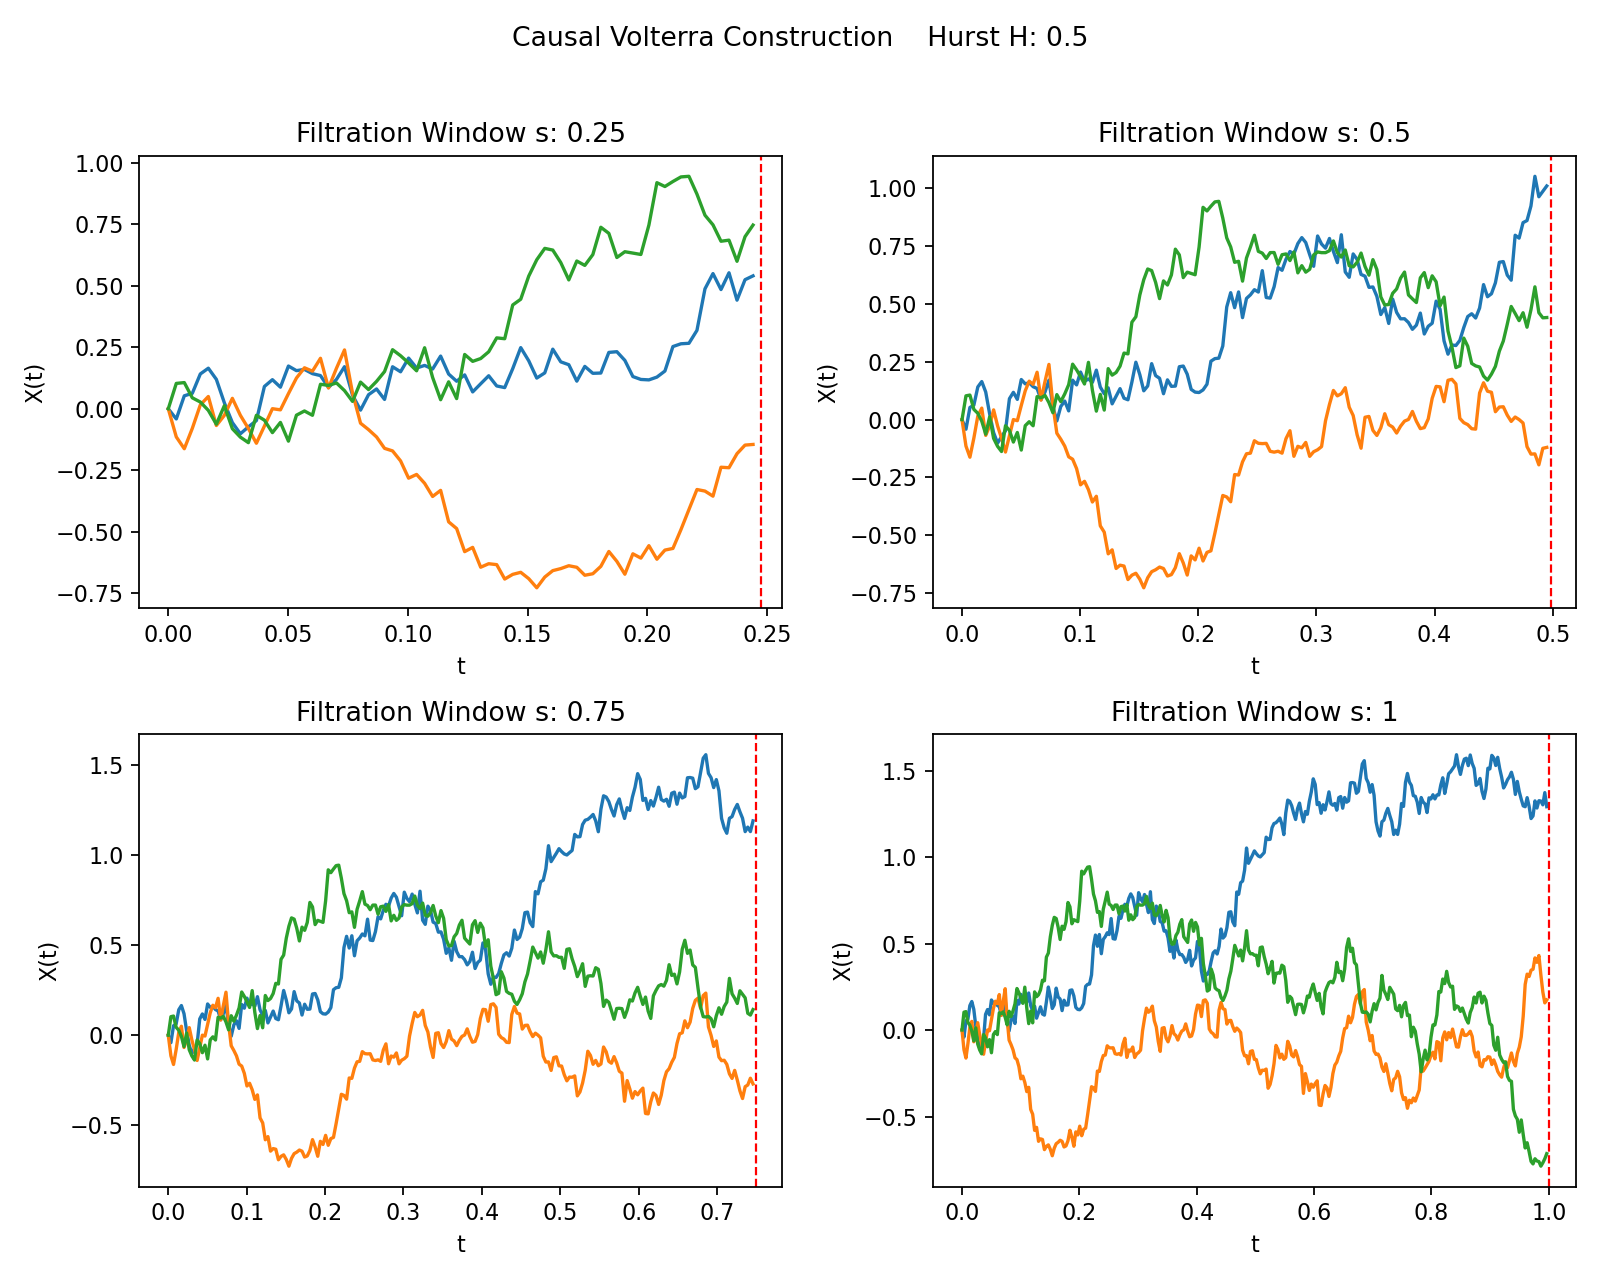
\includegraphics[width=\linewidth]{img/hft2-iterative0_5.png}
\end{minipage}
\hfill
\begin{minipage}[t]{0.54\textwidth}
\vspace{0.2cm}
\centering
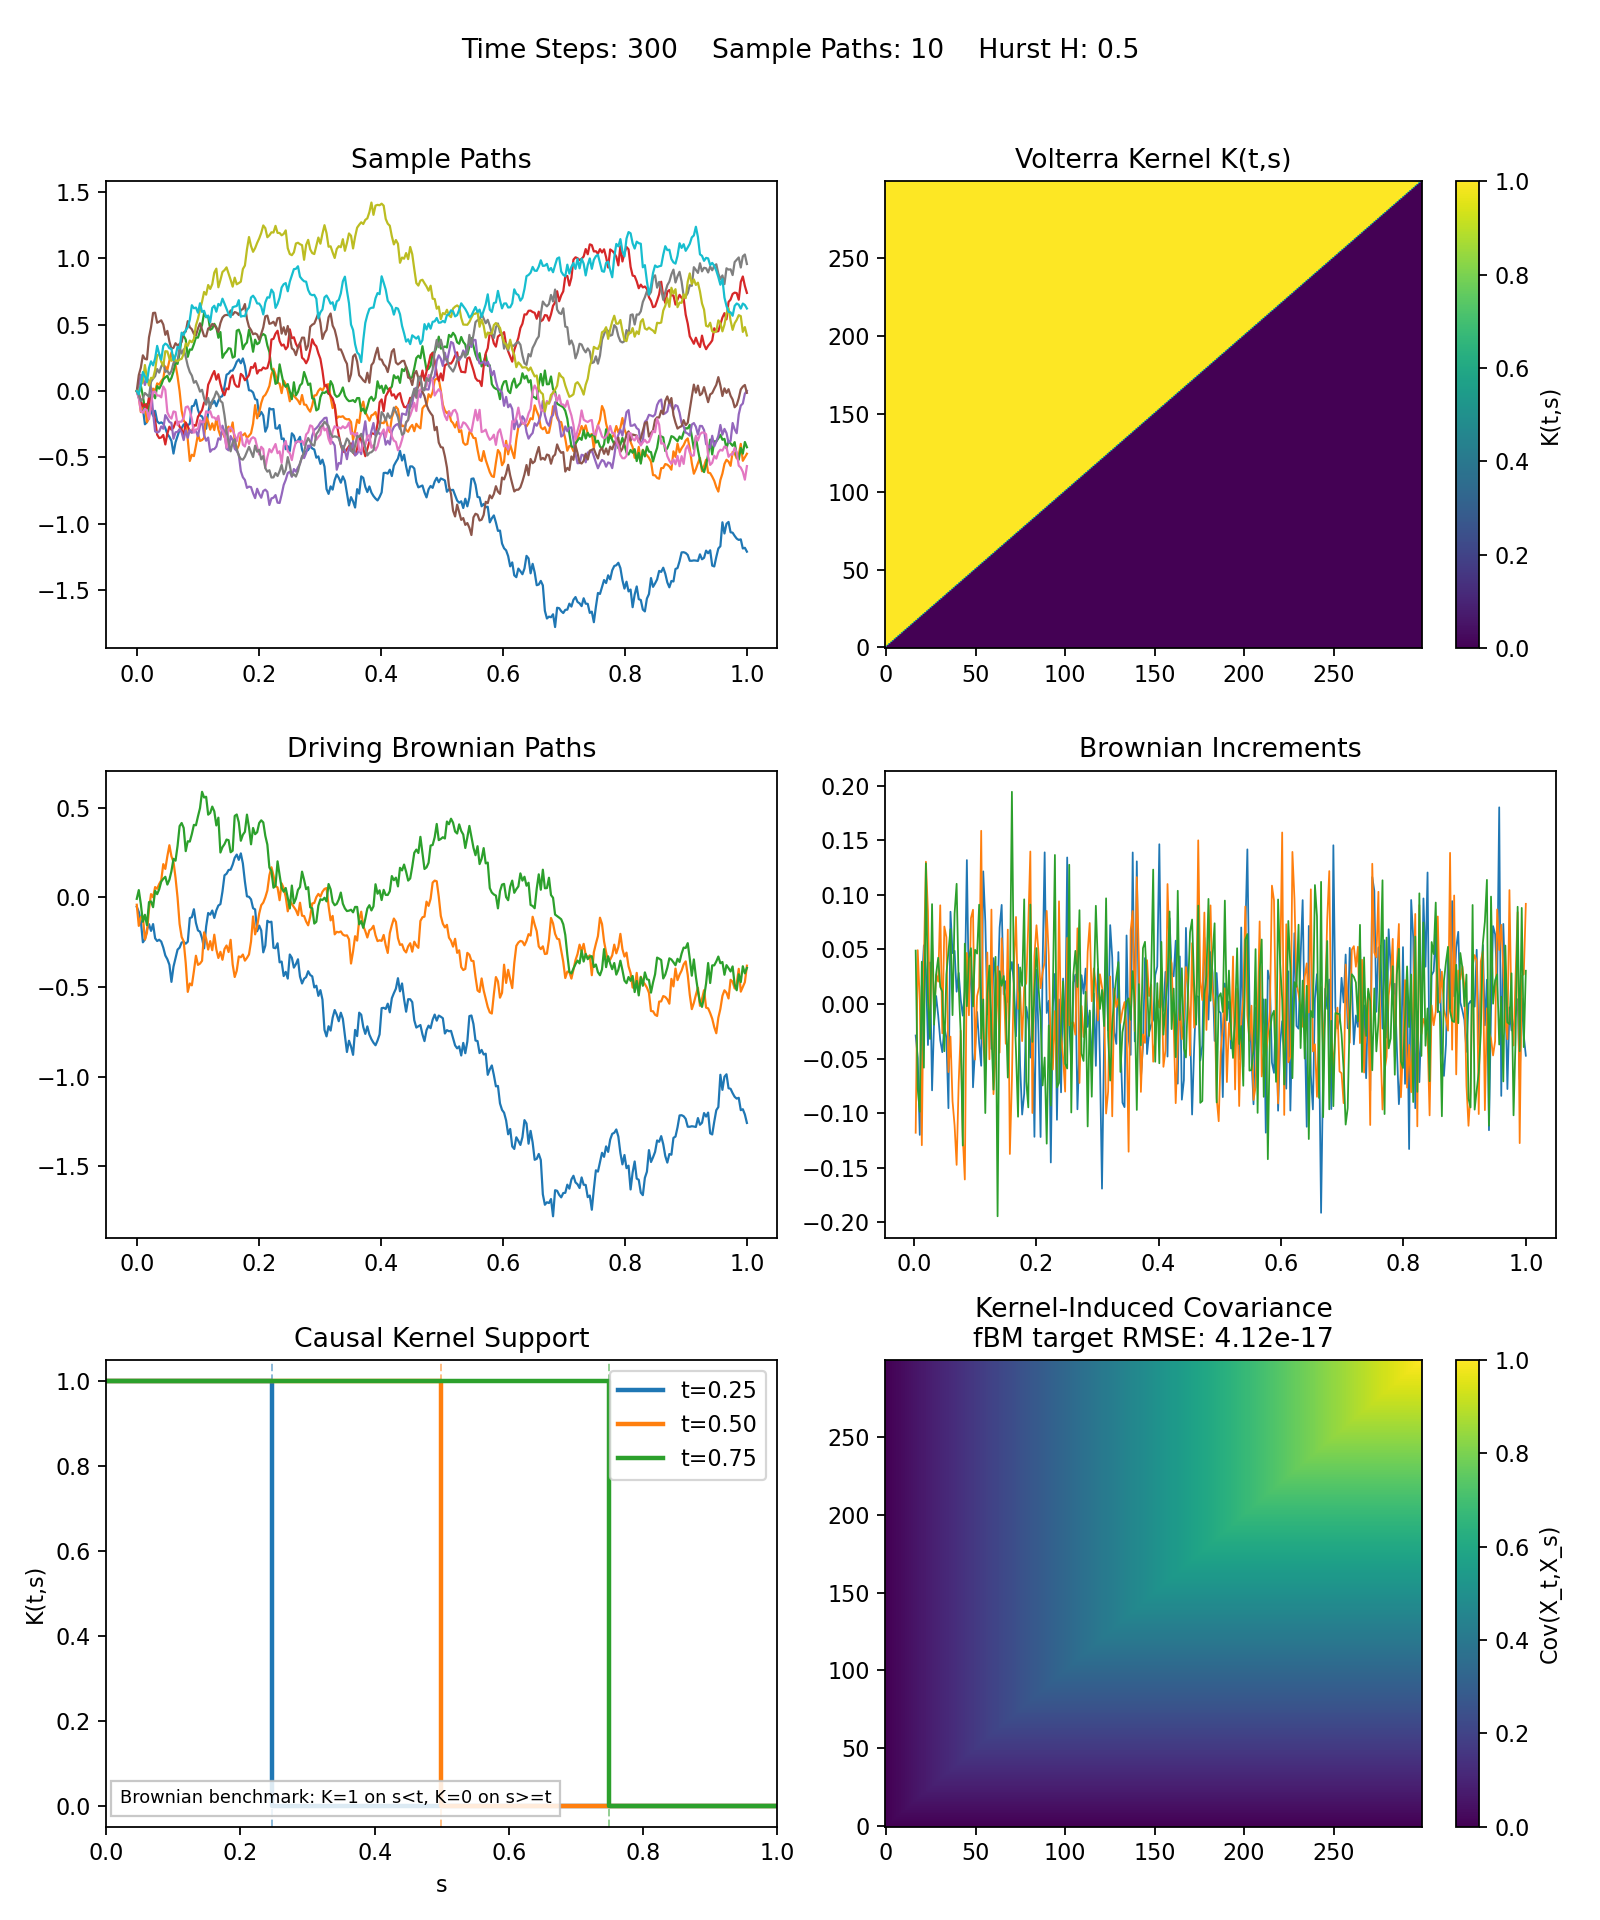
\includegraphics[width=\linewidth]{img/hft2-volterra0_5.png}
\end{minipage}
\end{figure}


\begin{figure}[H]
\centering
\begin{minipage}[t]{0.44\textwidth}
\vspace{0pt}
\normalsize
\textbf{Rough regime: \(H=0.2\).}

When the Hurst parameter is below $\tfrac12$ , the fractional-type kernel becomes more singular near the diagonal. This means that the process places a very large weight on the most recent shocks, while still retaining memory of the older ones. The iterative panels make this point visible: as the filtration window increases, the process is updated only from the observed past, but the contribution of the most recent increments remains dominant. 
This produces irregular, rapidly oscillating paths. 
Because the displayed power-law kernel is a tractable fractional-type prototype rather than the exact fractional-Brownian kernel, 
the covariance panel reports its 
discrepancy from the exact 
%fBM target instead of asserting equality.

\vspace{0pt}
\centering
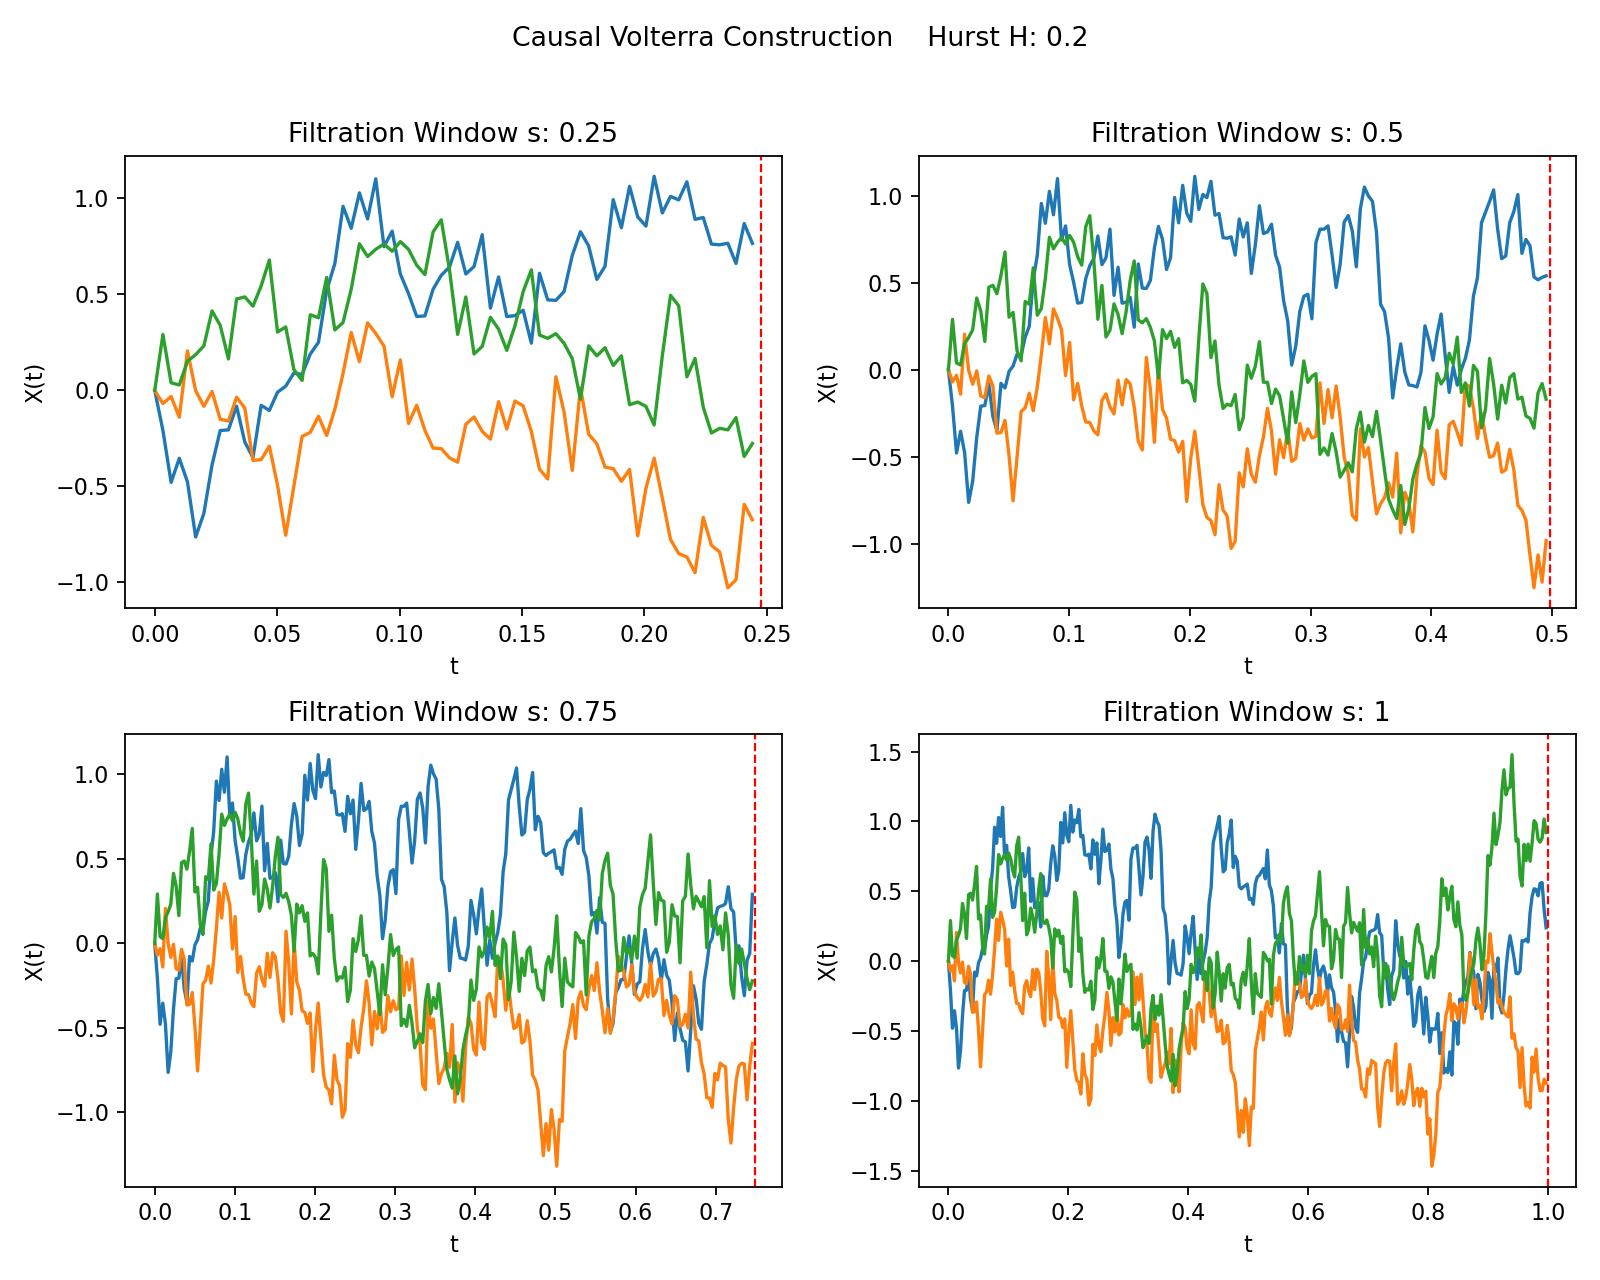
\includegraphics[width=\linewidth]{img/hft2-iterative0_2.png}
\end{minipage}
\hfill
\begin{minipage}[t]{0.52\textwidth}
\vspace{0pt}
\centering
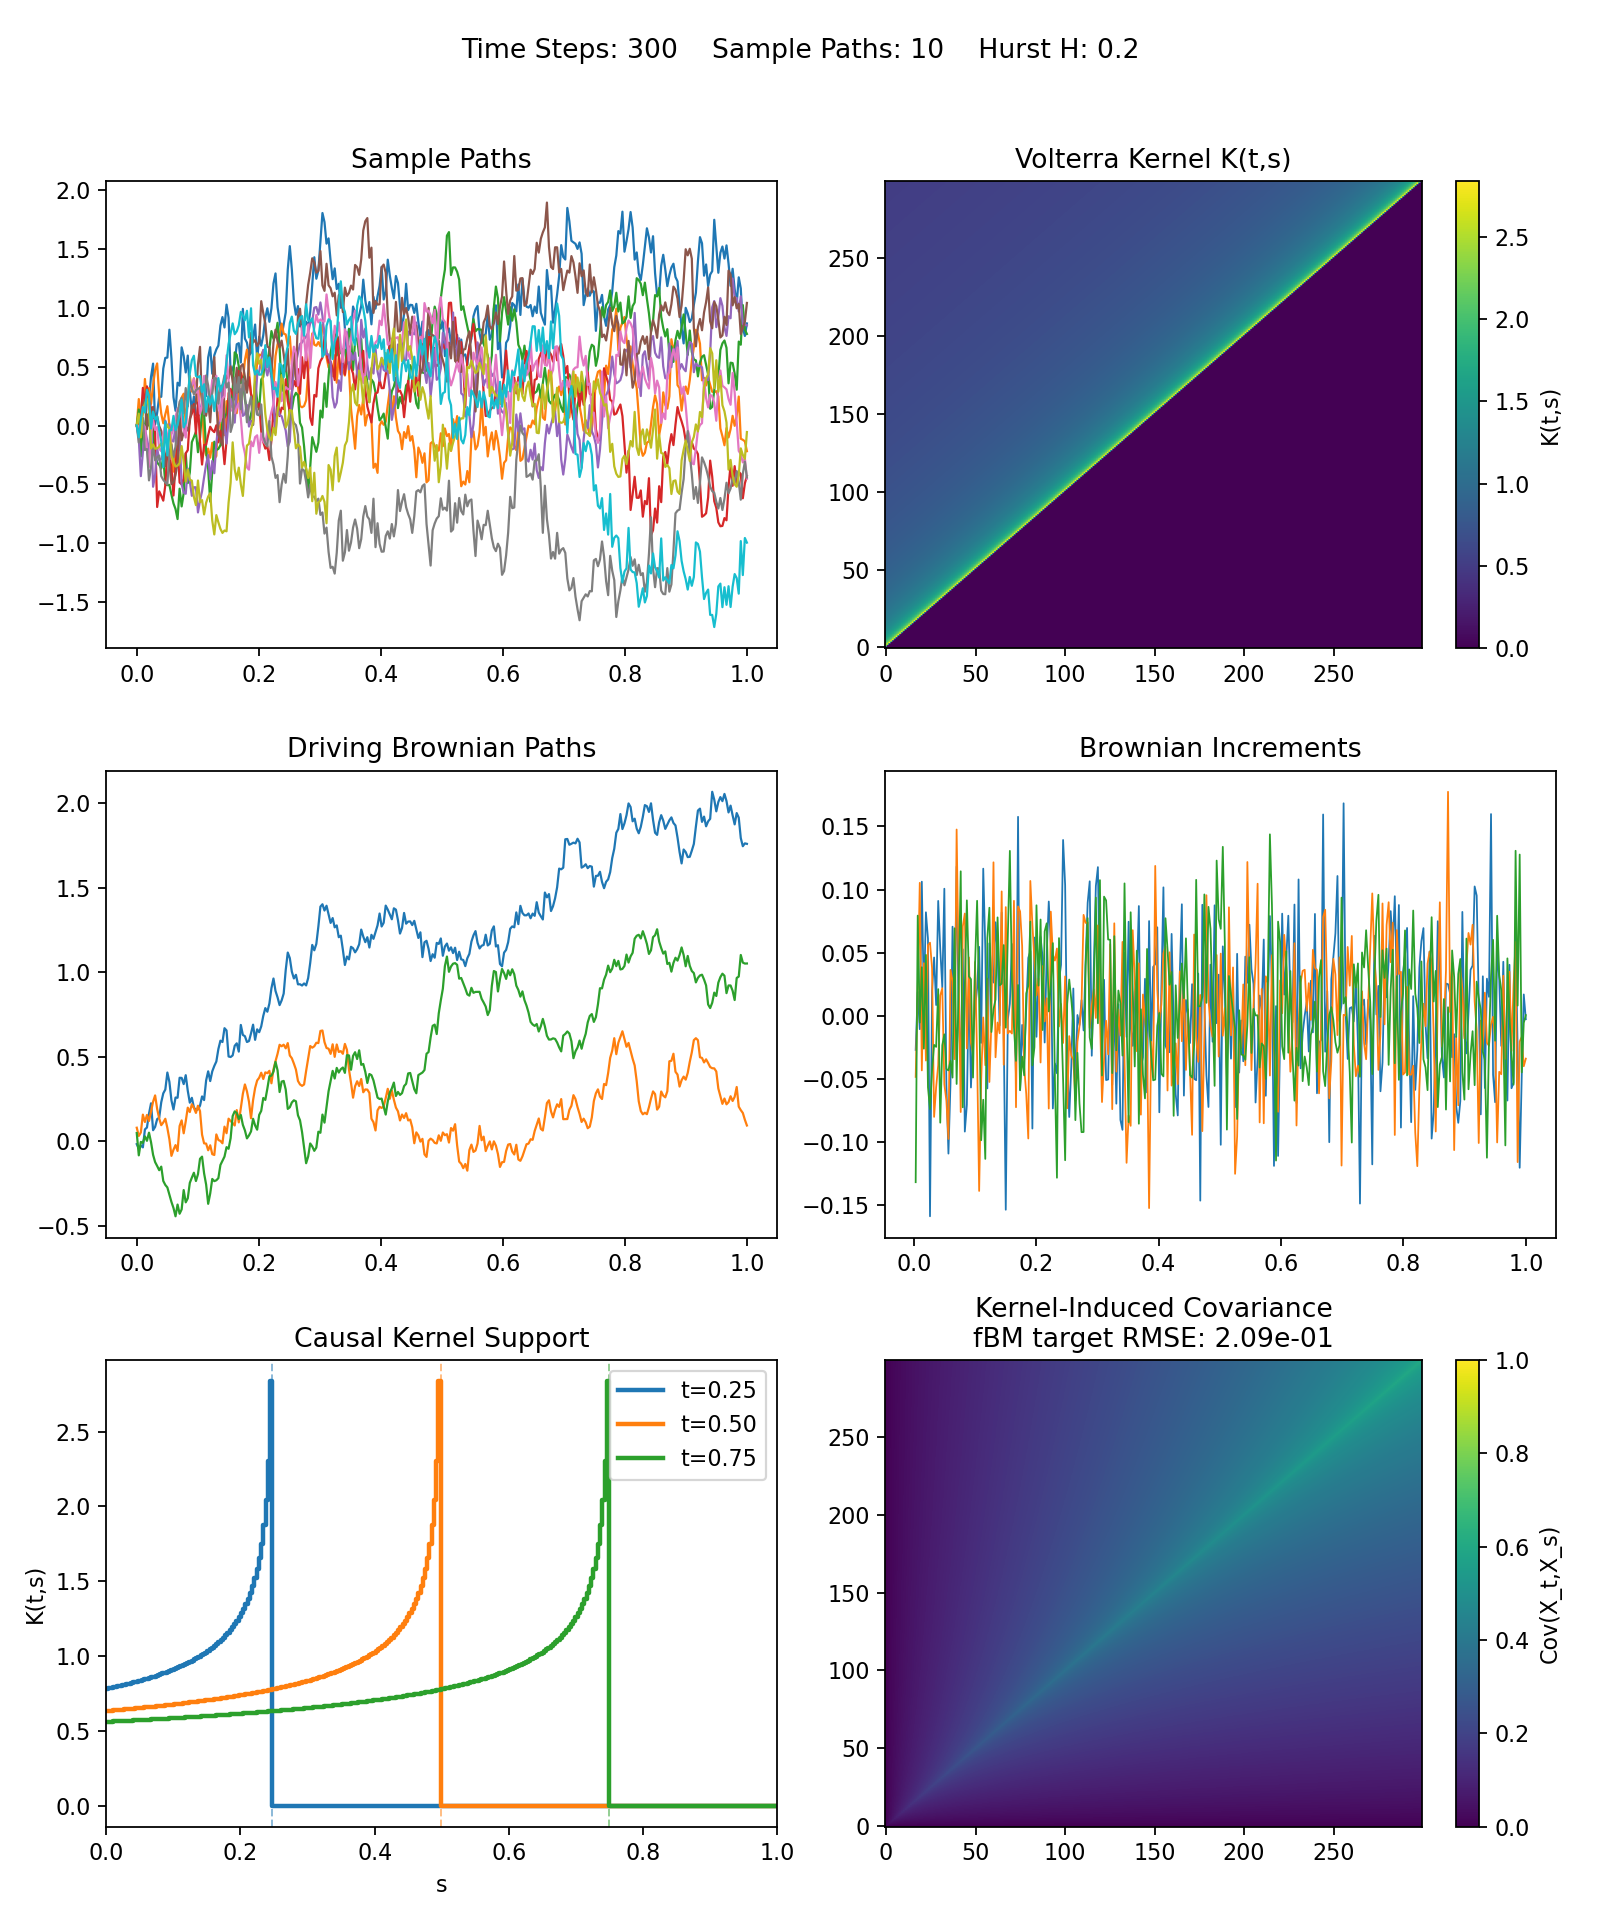
\includegraphics[width=\linewidth]{img/hft2-volterra0_2.png}
\end{minipage}
\end{figure}

\begin{figure}[H]
\centering
\begin{minipage}[t]{0.52\textwidth}
\vspace{0.4cm}
\centering
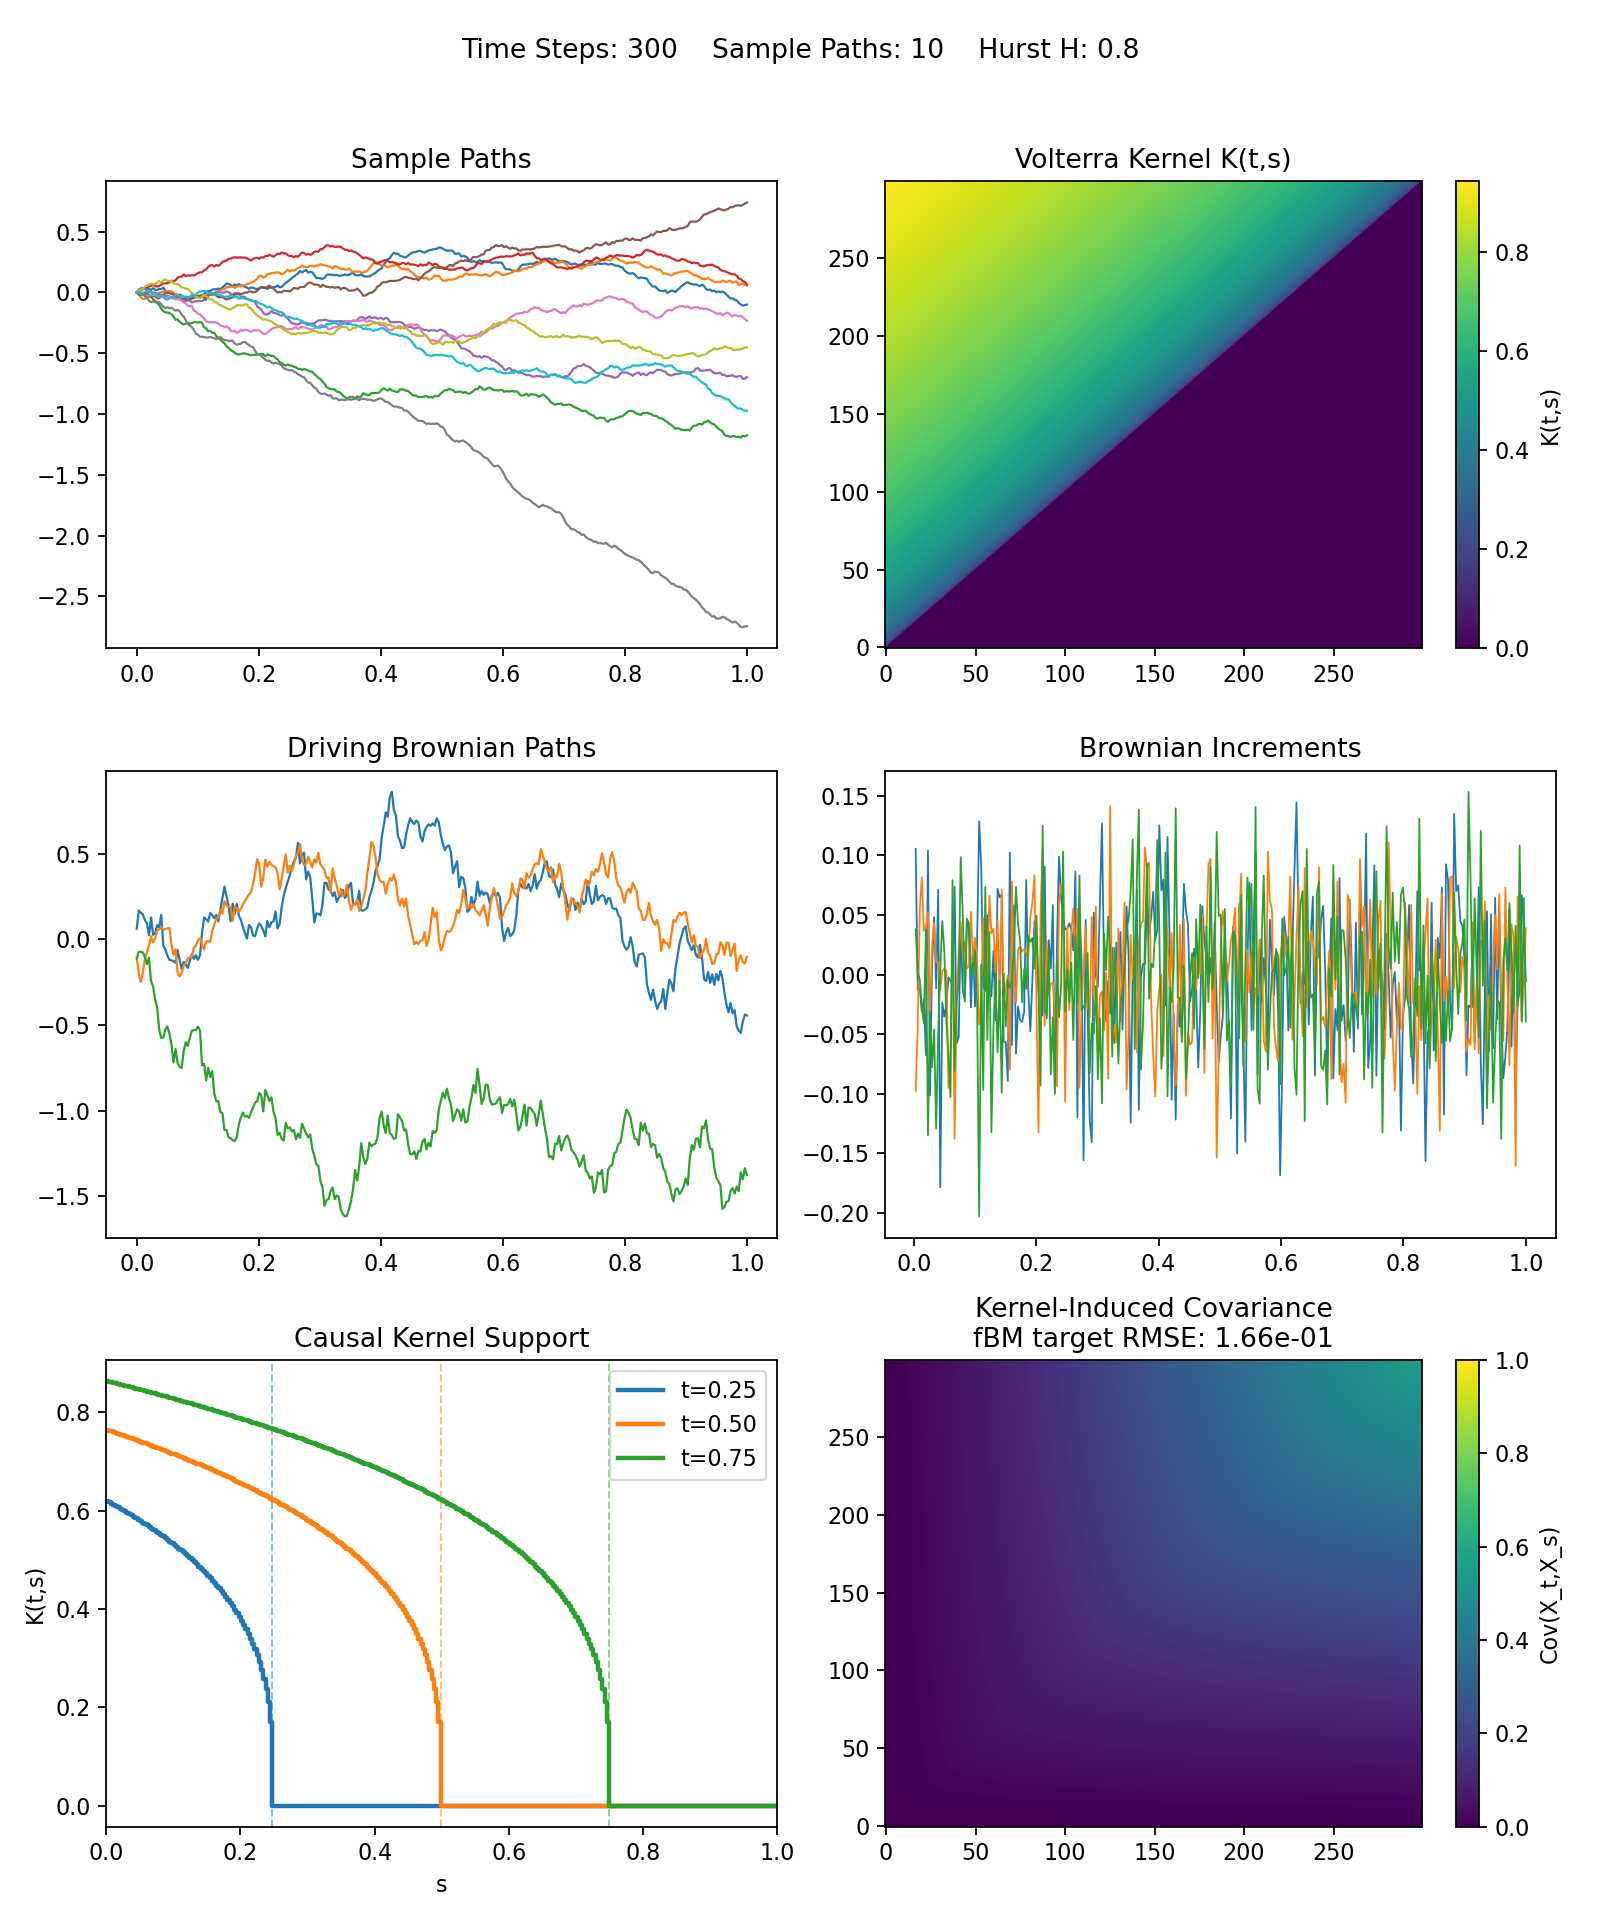
\includegraphics[width=\linewidth]{img/hft2-volterra0_8.png}
\end{minipage}
\hfill
\begin{minipage}[t]{0.42\textwidth}
\vspace{0pt}
\normalsize


\textbf{Persistent regime: \(H=0.8\).}

When \(H>\tfrac12\), the kernel becomes smoother and the relative importance of more distant history increases. The process still has a causal representation, since only past noise is used, but the accumulated effect of history now produces much smoother and more persistent trajectories. This is visible both in the iterative construction and in the full Volterra diagnostics: the paths display stronger directional continuity, and the covariance pattern becomes more persistent across time indices.

\vspace{0.5cm}
\centering
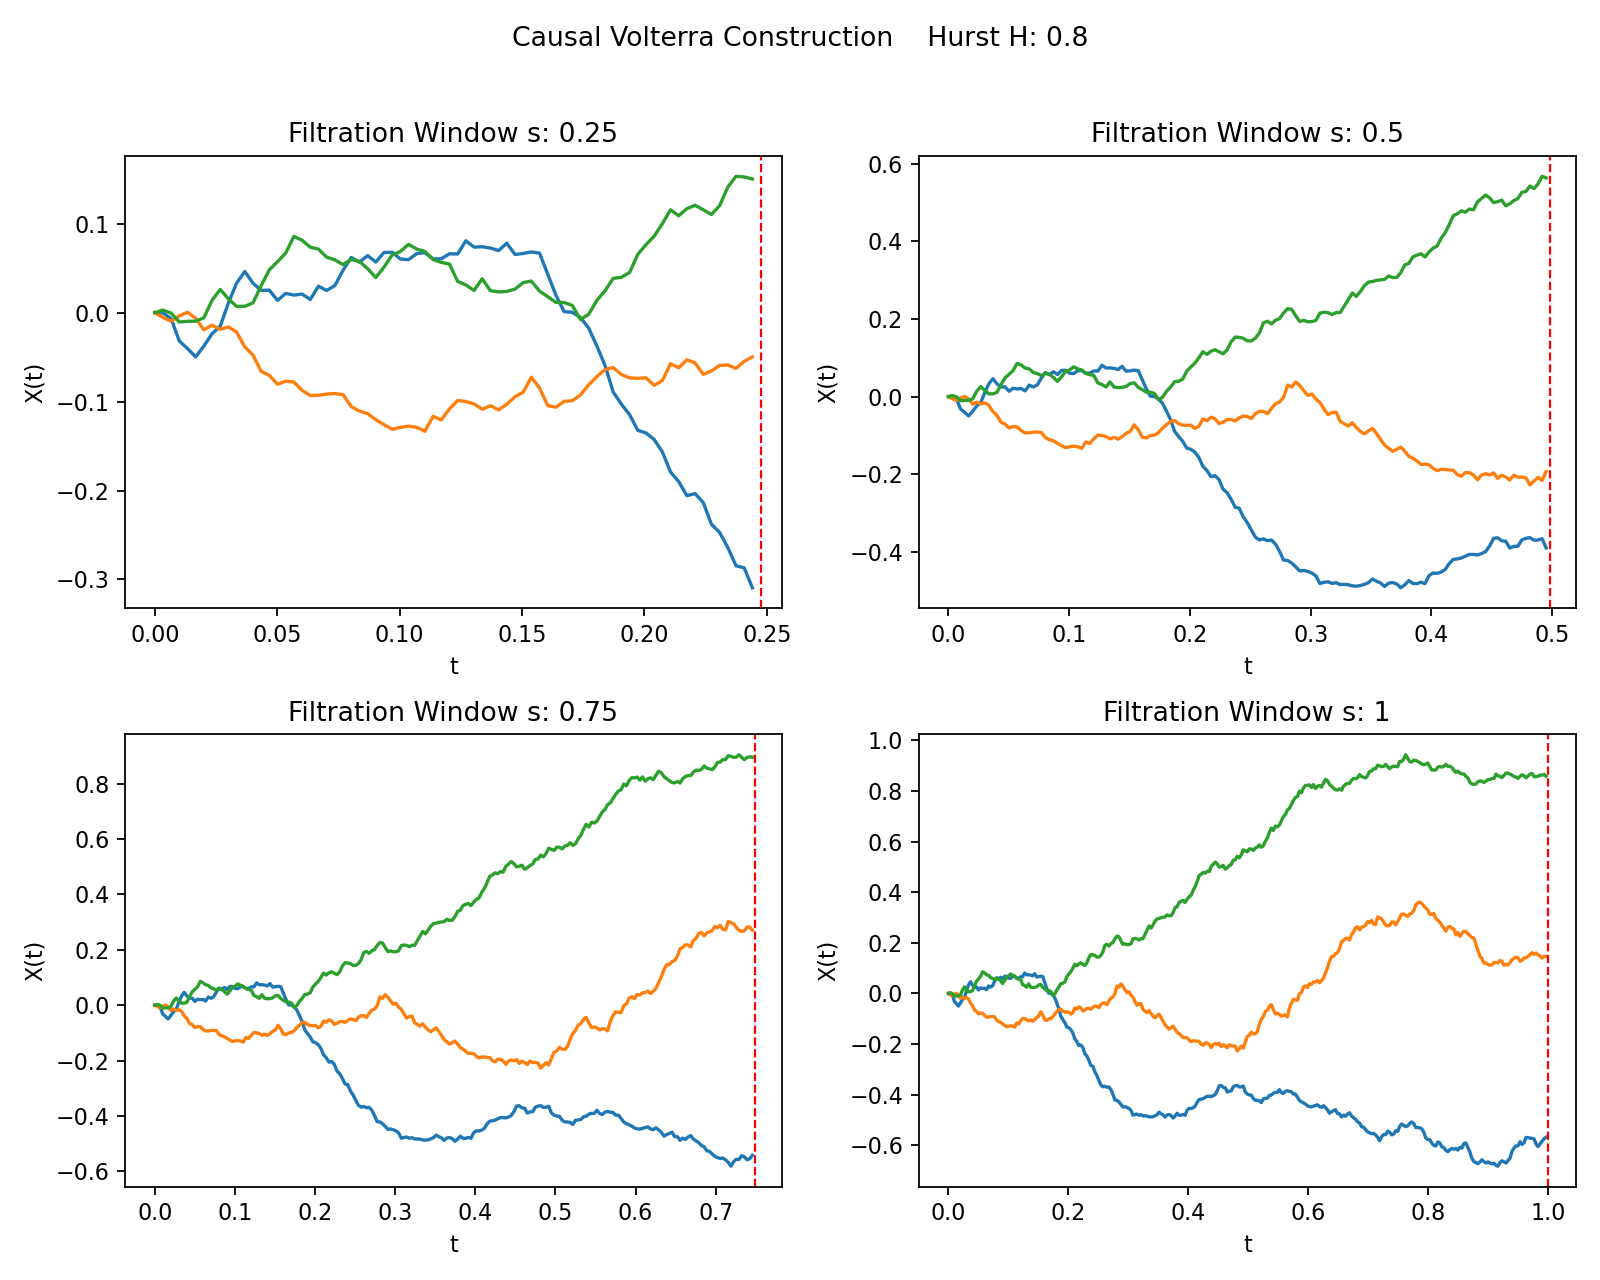
\includegraphics[width=\linewidth]{img/hft2-iterative0_8.png}
\end{minipage}
\end{figure}
\clearpage
\paragraph{Implementation.}

A convenient way to simulate a Volterra process numerically is to implement a generic routine that accepts a kernel as an argument. This makes it possible to recover Brownian motion, Ornstein--Uhlenbeck dynamics, or fractional-type processes simply by changing the kernel.

This implementation is intentionally generic. If one calls the simulator with \texttt{brownian\_kernel}, the output is a Brownian path written in Volterra form. If one uses \texttt{ou\_kernel(theta)}, the output becomes an Ornstein--Uhlenbeck process. If one uses \texttt{fractional\_kernel(H)}, the output is a causal fractional-type Volterra process whose roughness and persistence are controlled by \(H\).

\paragraph{Computational cost and transition to lifting.}

The Volterra representation solves the causality problem, but it does not eliminate the memory problem. To compute \(X_{t_i}\), one still has to survey the entire history of shocks \(\Delta W_0,\dots,\Delta W_{i-1}\). As a consequence, the cost per path grows roughly quadratically in the number of time steps:
\[
\text{cost per path} \sim O(n^2).
\]
This is acceptable for a theoretical laboratory and for moderate Monte Carlo experiments, but it becomes expensive once the process is embedded inside calibration loops, filtering procedures, or control problems.

The important gain is therefore structural rather than asymptotic: Volterra processes are causal, interpretable, and directly suited to sequential simulation. Their remaining computational bottleneck is exactly what motivates the next step of the paper. If the kernel can be approximated by a finite mixture of exponentials, the process can be rewritten in an enlarged but finite-dimensional Markovian state space. This is the idea behind Markovian lifting, which preserves the rough-memory intuition while recovering a tractable recursive structure for simulation and control.

%%%%%%%%%%%%%%%%%%%%%%%%%%%%%%%%%%%%%%%%%%%%%%%%
%%%%%%%%%%%%%%%%%%%%%%%%%%%%%%%%%%%%%%%%%%%%%%%%
%%%%%%%%%%%%%%%%%%%%%%%%%%%%%%%%%%%%%%%%%%%%%%%%

The singular-memory kernel is not solved by relabeling its scalar output as a Markov state. The next chapter replaces it by a finite sum of exponentials and retains all factor coordinates. This recovers recursion for the approximating model, while leaving the kernel approximation and any subsequent state compression visible.
